%%
%% Copyright 2007-2020 Elsevier Ltd
%%
%% This file is part of the 'Elsarticle Bundle'.
%% ---------------------------------------------
%%
%% It may be distributed under the conditions of the LaTeX Project Public
%% License, either version 1.2 of this license or (at your option) any
%% later version.  The latest version of this license is in
%%    http://www.latex-project.org/lppl.txt
%% and version 1.2 or later is part of all distributions of LaTeX
%% version 1999/12/01 or later.
%%
%% The list of all files belonging to the 'Elsarticle Bundle' is
%% given in the file `manifest.txt'.
%%

%% Template article for Elsevier's document class `elsarticle'
%% with numbered style bibliographic references
%% SP 2008/03/01
%%
%%
%%
%% $Id: elsarticle-template-num.tex 190 2020-11-23 11:12:32Z rishi $
%%
%%
\documentclass[preprint,12pt]{elsarticle}

%% Use the option review to obtain double line spacing
%% \documentclass[authoryear,preprint,review,12pt]{elsarticle}

%% Use the options 1p,twocolumn; 3p; 3p,twocolumn; 5p; or 5p,twocolumn
%% for a journal layout:
%% \documentclass[final,1p,times]{elsarticle}
%% \documentclass[final,1p,times,twocolumn]{elsarticle}
%% \documentclass[final,3p,times]{elsarticle}
%% \documentclass[final,3p,times,twocolumn]{elsarticle}
%% \documentclass[final,5p,times]{elsarticle}
%% \documentclass[final,5p,times,twocolumn]{elsarticle}

%% For including figures, graphicx.sty has been loaded in
%% elsarticle.cls. If you prefer to use the old commands
%% please give \usepackage{epsfig}

%% The amssymb package provides various useful mathematical symbols
\usepackage{amssymb}
%% The amsthm package provides extended theorem environments
%% \usepackage{amsthm}

\usepackage{cite}
\usepackage{amsmath,amssymb,amsfonts}
\usepackage{graphicx}
\usepackage{textcomp}
\usepackage{multirow}
\usepackage{hyperref}
\usepackage{booktabs}
\usepackage{algorithm}
\usepackage{algpseudocode}
\usepackage{subcaption}
\usepackage{lipsum} % For lipsum
\usepackage[dvipsnames]{xcolor} % Custom Colors
\definecolor{mygray}{gray}{0.6} % Definining a .6 transparency gray called mygray
\setlipsum{% Making the lipsum text mygray
  par-before = \begingroup\color{mygray},
  par-after = \endgroup
}
\newcommand{\tl}[1]{\textit{[{\color{red}#1}]}}
\newcommand{\cm}[1]{\textit{{\color{blue}#1}}}
\newcommand{\erik}[1]{\textit{[{\color{brown}Erik: #1}]}}
\newcommand{\mr}[1]{\textit{[{\color{brown}Mohammed: #1}]}}

\usepackage{lineno}

\journal{Future Generation Computer Systems}

\begin{document}

\begin{frontmatter}

%% Title, authors and addresses

%% use the tnoteref command within \title for footnotes;
%% use the tnotetext command for theassociated footnote;
%% use the fnref command within \author or \address for footnotes;
%% use the fntext command for theassociated footnote;
%% use the corref command within \author for corresponding author footnotes;
%% use the cortext command for theassociated footnote;
%% use the ead command for the email address,
%% and the form \ead[url] for the home page:
%% \title{Title\tnoteref{label1}}
%% \tnotetext[label1]{}
%% \author{Name\corref{cor1}\fnref{label2}}
%% \ead{email address}
%% \ead[url]{home page}
%% \fntext[label2]{}
%% \cortext[cor1]{}
%% \affiliation{organization={},
%%             addressline={},
%%             city={},
%%             postcode={},
%%             state={},
%%             country={}}
%% \fntext[label3]{}

\title{A Tiny, Human-interpretable, Client-side Classifier}

%% use optional labels to link authors explicitly to addresses:
%% \author[label1,label2]{}
%% \affiliation[label1]{organization={},
%%             addressline={},
%%             city={},
%%             postcode={},
%%             state={},
%%             country={}}
%%
%% \affiliation[label2]{organization={},
%%             addressline={},
%%             city={},
%%             postcode={},
%%             state={},
%%             country={}}

\author[1]{Charles Meyers}
\author[]{Aaron P. MacSween}
\author[1]{Tommy L\"{o}fstedt}
\author[1]{Erik Elmroth}

\affiliation[1]{organization={Department of Computing Science, Umeå University},%Department and Organization
            addressline={Universitetstroget 4},
            city={Umeå},
            postcode={90187},
            state={Västerbotten},
            country={Sweden}}
% Note, that the above section breaks if I use \aa for Umea or \"{a} for Vasterbotten


\begin{abstract}
%% Text of abstract
The recent developments in machine learning have highlighted a conflict between online platforms and their users in terms of privacy.
The importance of user privacy and the struggle for power over their data has been intensified as regulators and operators attempt to police the platforms.
As users have become increasingly aware of privacy issues, client-side data storage, management, and analysis have become a favoured approach to large-scale machine learning.
State-of-the-art machine learning methods require vast amounts of labelled user data, making them unsuitable for models that reside client-side and only have access to a single user's data.
State-of-the-art methods are computationally expensive, which degrades the user experience on compute limited hardware and also reduces battery life.
Classical machine learning methods often require fewer samples to be effective, but may not provide the same performance as large-scale neural networks, for instance.
A recent alternative approach has proven remarkably successful in classification tasks across a wide variety of data---using only a small number of samples. The idea is to use compression to measure the distance between objects in classical distance-based machine learning methods.
In this work, we present techniques to improve the run-time characteristics of this compression-based metric, denoted normalized compression distance, and develop it for the wider context of kernel methods to allow modelling complex data using only a small number of samples.
We show that the compression metric outperforms other string metrics and kernel methods---without incurring additional computational costs.
The end results is a simple, client-side, classification model with an accuracy that competes with state-of-the-art models while using only a fraction of their power, data, and compute requirements---with training times measured in seconds instead of days or weeks.
\end{abstract}

%%Graphical abstract
\begin{graphicalabstract}
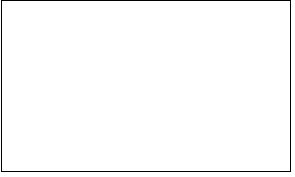
\includegraphics{grabs}
\end{graphicalabstract}

%%Research highlights
\begin{highlights}
\item Research highlight 1
\item Research highlight 2
\end{highlights}

\begin{keyword}
%% keywords here, in the form: keyword \sep keyword
keyword one \sep keyword two
%% PACS codes here, in the form: \PACS code \sep code
\PACS 0000 \sep 1111
%% MSC codes here, in the form: \MSC code \sep code
%% or \MSC[2008] code \sep code (2000 is the default)
\MSC 0000 \sep 1111
\end{keyword}

\end{frontmatter}

\linenumbers

%% main text
\section{Introduction}

Despite their efficacy across many domains, modern machine learning (ML) methods often have large numbers of parameters, and thus also require large numbers of samples to train~\cite{desislavov2021compute}.
In the context of online platforms, data are collected from end-users using dubious amounts of consent~\cite{nouwens2020dark} and aggregated at massive scales~\cite{desislavov2021compute}.
Such data collection on online platforms often creates privacy and security risks~\cite{chakraborty_adversarial_2018,meyers}.
Examples of privacy risks include attempts by regulators to weaken encryption standards~\cite{amnesty_encryption} or platform operators using ML to scan client devices for offensive content~\cite{chat_control}, leading to risks of private data leaks~\cite{xiao2021improving,fredrikson_model_2015} while at the same time being trivial to circumvent by malicious actors~\cite{carlini_towards_2017,dohmatob_generalized_2019,hopskipjump,biggio_evasion_2013,meyers,chakraborty_adversarial_2018,trashfire}.

\subsection{Threat Model}
\label{threat}
Current platform solutions often rely on large-scale ML methods that are trained on vast amounts of user data and federated across devices~\cite{apple_csam}---an approach that has been criticized by privacy experts~\cite{abelson2024bugs}.
Examples of security risks include attacks against ML systems that target a model during training~\cite{biggio_poisoning_2013}, prediction~\cite{biggio_evasion_2013,deepfool,carlini_towards_2017}, and deployment~\cite{distributed_attacks,santos2021universal}.
Even when access to a model by an adversary is limited, it is possible to induce a misclassification~\cite{hopskipjump}, reverse engineer the model~\cite{extraction_attack}, determine the model weights~\cite{jagielski2020high}, or infer the class-membership of new samples~\cite{bentley2020quantifying}.
This raises profound questions for safety-critical systems~\cite{meyers} and legal questions about access and control of the underlying data~\cite{mitrou2018data,marks2023ai}.
Additionally, it has been shown that finding prototypical meta samples from the training set of large-scale ML models is trivial~\cite{chakraborty_adversarial_2018}.
Even if the attacker only has access to a typical application programming interface (API), there are reliable ways to fool the model~\cite{hopskipjump}.
In short, distributed and centralised training paradigms are both inherently fragile to malicious users and dangerous for user privacy, even if the resulting model lives on the user device (rather than in the cloud).

Instead of relying on a model trained on massive amounts of user data, as is typical in large-scale ML applied to platform-level data, it is possible to categorically sidestep the aforementioned attacks with a model that runs entirely client-side.
By avoiding the typical model-as-a-shared-service approach, the attack surface is reduced to only adversaries that have access to data that users generally consider private (\textit{e.g.}, the contents of a message).
That is, the attack surface is reduced and can be unique to each user, session, or device by using data from each user in isolation and training a model on that user's device. Client-side models would only need to share a single bit (the classification label in a binary classification context) with the platform operator---allowing those operators to serve user-specific contents without exfiltrating private data from their entire user base.
However, not training a model on large amounts of collected user data means that such hypothetical client-side methods are at risk of not performing at the level of state-of-the-art large-scale methods.

Recently, Jiang \textit{et al.}~\cite{jiang2022less} proposed a remarkably successful approach: a parameter-free text classification method (denoted NCD-KNN) that exploits a compression-based distance measure, the \textit{normalized compression distance} (NCD)~\cite{ncd}, to classify objects using the k-nearest neighbours (KNN) method~\cite{shalev2014understanding}.
We limit ourselves to strings here because some of the datasets are string data and the others are formatted as such for the experiments to allow for direct comparisons across all of the datasets.
To use NCD, the model builder must choose a compression algorithm.
While the effect of various compressors has been explored, in part, before~\cite{ncd_pitfalls}, but we expand the analysis in \cite{ncd_pitfalls} to newer compression algorithms and offer additional run-time improvements over Jiang \textit{et. al's} method.
The NCD-KNN method has shown very strong performance across several benchmarks, but their implementation was not appropriate for real-time settings.
However, NCD is a pseudo-metric~\cite{opitz2023gzip, weinreich2023parameter, nishida2011tweet, jiang2022less}, which means that applying ML methods blindly can lead to erroneous results (\textit{e.g.} by incorrectly ordering the nearest neighbours).
In this work we compile some examples of this pseudo-metric behaviour Section~\ref{pseudometric} and propose techniques to mitigate the effects of this behaviour in Section~\ref{improvements}.
We also propose run-time improvements over Jiang~\textit{et. al.'s} method (Section~\ref{improvements}).
Additionally, we expand the notion of NCD-as-a-distance~\cite{opitz2023gzip,weinreich2023parameter,nishida2011tweet,ncd,jiang2022less} to kernelised models (Section~\ref{kernels}) in an attempt to model more complex decision boundaries than those allowed by KNN.
That is, we extend this notion of distance (dissimilarity) to one of kernel-like similarity; offer run-time improvements over Jiang's method~\cite{jiang2022less};
and demonstrate the efficacy of our run-time optimised method on a variety of datasets to produce a model that is as accurate as state-of-the-art ML models trained on much larger datasets.



\subsection{Motivations}

There are several motivations for this work.
First, \textit{normalized compression distance} (NCD) has been demonstrated to be a \textit{universal} measure of similarity between two objects~\cite{ncd}.
Secondly, Jiang's analysis~\cite{jiang2022less} relies on many thousands of samples, which would be unsuitable for the proposed (client-side) implementation and their algorithm includes unnecessary, repeated calculations.
Additionally, it's unclear how well Jiang's method performs in few-shot circumstances or in the case of extremely imbalanced data (\textit{e.g.}, malicious user datasets).
While other research examined topics like image classification~\cite{opitz2023gzip}, chemical classification~\cite{weinreich2023parameter}, and text classification~\cite{nishida2011tweet}, the ability of NCD to classify tabular data remains largely unexplored.

However, the original work includes an error term that is subsequently ignored by recent research ~\cite{opitz2023gzip,weinreich2023parameter,nishida2011tweet,jiang2022less}, despite it appearing in the original formulation~\cite{ncd}.
To the best of our knowledge, no research has addressed the problem of negative values for NCD as the original authors~\cite{ncd} insist that this measure is always positive. % The \@ signals to the linter that this is the end of a sentence and not an abbreviation. The linter can also handle stuff like \textit{e.g.} vs e.g. vs eg, hyper-parameter vs hyperparameter, etc. It's very useful and doesn't make automated changes (like a python linter would).
This is clearly demonstrated to be false in Section~\ref{pseudometric}.

Also, these prior works focus on distance-based algorithms  (\textit{e.g.} KNN), restricting our classification boundary to relatively simple geometries.
We extend this technique to reproducing kernel Hilbert spaces and thus more elaborate ML methods---allowing for more complex decision boundaries.
Furthermore, if run-time storage and computation requirements are minimised, then we can fulfill our goal of deploying this method entirely client-side.
In the simplest case, that might mean marking an email as spam~\cite{ansuz_email} or examining the nearest neighbours of a sample in a browser~\cite{ansuz_browser}.
The goal of the work is to explore the efficacy of NCD in the context of kernelised classifiers and produce a human-interpretable model with state-of-the-art accuracy that can be trained on and used by each user in isolation from all others, categorically circumventing the privacy and security concerns associated with the collection and analysis of millions of user-generated data points.



\subsection{Contributions}
In this study, we:

\begin{itemize}
    \item Demonstrate that normalized compression distance is a pseudo-metric (Section~\ref{pseudometric}) and propose techniques to mitigate the effects of this (Section~\ref{extensions}).
    % \item Discuss how private model deployment is safer by design (Section~\ref{threat}) and the efficacy of this design-constraint on several datasets (see Figure~\ref{fig:sample_size}).
    \item Develop a classifier (with KNN, logistic regression, or SVC) that offers large run-time improvements over NCD-KNN (Section~\ref{improvements}).
    \item Provide efficient implementations of the proposed classifiers in \texttt{javascript} as well as a \texttt{scikit-learn} compatible implementation in \texttt{Python} .
    \item Evaluate and empirically show the efficacy of the proposed compression-based classifiers across several binary classification datasets.
\end{itemize}





\section{Background}

In the sections below, we describe and define the NCD, summarize existing string metrics, briefly explore the run-time of KNN classifiers, and give a high-level overview of relevant compression algorithms.



\subsection{Measures of Distance}

This section outlines the distance measures outlined in this work.
In addition to the proposed metric (NCD), the accuracy and run-time characteristics of several string metrics are examined.
To model datasets that are comprised of strings, several measures of distance between strings are routinely used~\cite{levenshtein}.
For numeric data, other metrics can be used.
The set of evaluated string metrics is outlined below in Section~\ref{string_metrics}.
A somewhat forgotten method (NCD), proposed in 2001~\cite{ncd} (see Section~\ref{ncd}), extends to any type of object (not just strings).
Jiang \textit{et al.}~\cite{jiang2022less} proposed to use NCD in conjunction with the KNN classifier, but this idea can be extended to other classifiers (\textit{e.g.} SVCs~\cite{vapnik1994measuring}) that use measures of distance to cluster samples into classes.


\subsubsection{Normalized Compression Distance}
\label{ncd}

The normalized compression distance~\citep[NCD;][]{ncd} is defined as
\begin{equation}
    \text{NCD}(x, y) = \frac{\mathcal{C}(xx') - \min\{\mathcal{C}(x), \mathcal{C}(x')\}}{\max\{\mathcal{C}(x), \mathcal{C}(x')\}} + \varepsilon,
\end{equation}
where $\mathcal{C}(z)$ is the length (in bits) of the compressed form of the data, $z$, using a compression algorithm, $\mathcal{C}$, the notation $xx'$ denotes the concatenation of strings $x$ and $y$, and $\varepsilon$ is an error accounting for imperfect compression algorithms~\cite{ncd}. This error is generally assumed to be small relative to the rest of the terms, but, as the original authors already noted, the resulting NCD values may be larger than one~\cite{ncd}.



\subsubsection{Other measures of string distance}
\label{string_metrics}

To evaluate the relative performance of the NCD metric defined above, we compare it to several common measures of string similarity, and these are briefly outlined below.
% String Distances
\begin{itemize}
    \item \textit{Levenshtein:} is the ``edit distance'' or minimum number of single-character edits to transform one string into another~\cite{navarro2001guided}.
    \item \textit{Ratio:} is the Levenshtein distance divided by the total length of the strings~\cite{levenshtein}.
    \item \textit{Hamming:} is the number of character positions where two strings differ.
\end{itemize}

%  Working on fomrulat definitions here
% Hamming: d_{Hamming}(x, x') = \sum_{i=1}^{n} \mathbb{1}_{\{x_i \neq x'_i\}},
% d(x, x') = \text{lev}(x, x') = \min \begin{cases}
% d(x_1, x'_1) + \mathbb{1}_{\{x_1 \neq x'_1\}} & \text{(substitution)} \\
% d(x_1, x') + 1 & \text{(deletion)} \\
% d(x, x'_1) + 1 & \text{(insertion)}
% \end{cases}
%  d_{ratio} = (d_{Levenshtein} / (l(x) + l(x'))
% d(x, x') = \frac{1}{3} \left( \frac{M}{|x|} + \frac{M}{|x'|} + \frac{M - t}{M} \right)
% where $M$ is the number of matching characters in the two strings and $T$ is the number of transposed characters


\subsubsection{Metric Spaces}
\label{metric_spaces}
A metric space is defined by some measure of distance ($d:X \times X \rightarrow \mathbb{R}$) between the constituent components of some space, usually called points.
We denote the points $x_1,x_2,\ldots,x_n$  in a set $X$, separated by distance $d(x_1,x_2)$, where  $\mathbb{R}$ denotes the set of real numbers.
The distance function, $d$, is said to be a \textit{proper} metric if the following four axioms are satisfied for all points in $X$~\cite{metrics}:

\begin{itemize}
    \item $d(x_1,x_2) = 0 \iff x_1 = x_2$ (zero axiom)
    \item $d(x_1,x_2) \geq 0$ (non-negativity axiom)
    \item $d(x_1,x_2) = d(x_2, x_1)$ (symmetry axiom)
    \item $d(x_1, x_3) \leq d(x_1,x_2) + d(x_2,x_3)$ (triangle inequality axiom).
\end{itemize}

\subsection{Notation}
We denote the cardinality of a set, $X$, as
$$
    | X |.
$$
For a matrix, $D$, $D_{ij}$ is the entry of $D$ at the $i$-th row and $j$-the column.

\subsubsection{Kernelisation}
\label{kernels}

Whereas distance functions are used to measure the \textit{dissimilarity} between different examples, $x,x'$, a \textit{kernel-function}, $K$, is a measure of \textit{similarity}.
We can use NCD to construct (or, at least, approximate) a kernel, allowing it to be used with a much larger set of ML methods than as a distance.
The kernel functions that were evaluated in this work are defined in the next paragraphs.



\paragraph{Quadratic Kernel}
\label{quadratic_kernel}
The quadratic kernel~\cite{kernels} maps the input data to a higher-dimensional space by considering the pairwise quadratic interactions between the features of the input vectors.
The quadratic kernel is defined as
$$
    k(x, x') = (s \cdot d(x,x') + c)^2,
$$
where $x$ and $x'$ are two vectors in the input space, and $s, c$ are tunable parameters.
\cm{TODO: test more parameters for this kernel}



\paragraph{Multiquadric Kernel}
\label{multiquadric_kernel}
The multiquadric kernel~\cite{kernels} provides one another non-linear mapping.
It is defined as
$$
k(x, x') = \sqrt{d(x,x') ^2 + c^2}
$$
where $c$ is a tunable constant.


\paragraph{Exponential}
\label{exp_kernel}

Another kernel function is the exponential kernel~\cite{kernels}, defined by
$$
    k(x, x') = \exp\left\{-\frac{d(x,x')}{\gamma}\right\},
$$
where $\gamma$ is a tunable parameter (called a length scale) that controls the rate of similarity decay between dissimilar samples. In order to use these methods with NCD, the pairwise distances between all samples must first be calculated and stored as a matrix, generally called a \textit{distance matrix}.



\subsection{Calculating the distance matrix}
\label{distance_matrix}

To use ML methods on string data, it must be converted to a numeric representation.
To accomplish this, we calculate the pairwise distances between two sets of samples (denoted $X, X'$) to generate a \textit{distance matrix} ($D$), as outlined in Algorithm~\ref{alg:vanilla} (though we propose modfications to this algorithm in Section~\ref{modifications}).
For the training step, $X = X'$ and, for prediction, it is assumed that $X \neq X'$.
While many of the above distance metrics are symmetric, this is not necessarily the case with NCD and this distance matrix must be calculated for all pairs of samples $\{(x_i, x_j) \mid x_i \in X, x_j \in X'\}$.
Algorithm~\ref{alg:vanilla} clearly shows that the run time associated with finding the distance matrix scales with the cardinality of sets, denoted $n = | X |, m = | X' |$, such that the run time is $\mathcal{O}(nm)$ for both compute and memory.
\begin{algorithm}
    \begin{algorithmic}
        \Require Datasets $X$, $X'$ and some distance function $d(x,x)$.
        \For{$x_i \in X$}
            \For{$x_j \in X'$}
                \State $D_{ij} \gets d(x_i, x_j)$
            \EndFor
        \EndFor
        \State \Return Distance matrix $D$ with dimensions $m,n$.
    \end{algorithmic}
    \caption{Compute the ``Vanilla'' Distance matrix}
    \label{alg:vanilla}
\end{algorithm}

Clearly, if the number of samples in $X$ or $X'$ is large, then run-time becomes a major concern as the run-time requirements scale with the cardinality of the training set $m = | X | $ as well as the test set, $n = | X' |$, giving a run-time of $\mathcal{O}(mn)$ for calculating the distance matrix.
While KNN can avoid a training step entirely, if other models like logistic regression or support vector classifiers (SVCs) are desired, then training consists of finding the distance matrix $D_{i,j} = d(x_i, x_j) \forall i,j$ in a training set $X$, yielding a run-time of $\mathcal{O}(m^2)$ for training.
Letting $X'$ be the set of unlabelled samples (\textit{e.g.} a test set), then finding the distance matrix between for $X,X'$ has a complexity of  $\mathcal{O}(mn)$ for both run-time and memory.
Run-time improvements for calculating this distance matrix are considered in Section~\ref{improvements}.

\subsection{Calculating the distance matrix}
\label{gram_matrix}

To calculate the kernel matrix $ K(X, X') $, we start by computing the pairwise distances between the samples in $ X $ and $ X' $, as outlined in the subsection above.
The distance matrix $ D $ contains the values $ D_{ij} = d(x_i, x_j) $ for all pairs of samples $ x_i \in X $ and $ x_j \in X' $. The kernel matrix $ K(X, X') $ is then derived by applying a kernel function $ K(x_i, x_j) = k(d(x_i, x_j)) $, where $ k $ is a function that transforms the distances into similarities.




\subsection{NCD-KNN}
\label{ncd-knn}

A recent paper introduced NCD as a ``parameter-free'' measure of distance for the KNN classifier~\cite{jiang2022less}, though NCD as a measure of distance dates back two decades~\cite{ncd}.
However, some pairs of strings yield NCD distances that do not follow the axioms listed in Section~\ref{metric_spaces}, particularly when the strings are very short or the number of unique symbols (\textit{i.e.} alphabet) in those strings is very small (see Section~\ref{pseudometric} and Figures~\ref{fig:synthetic_check}~and~~\ref{fig:real_world_check}).
Section~\ref{pseudometric} details some string pairs that induce improper distances and Section~\ref{improvements} details the proposed mitigations and improvements.
The results in Section~\ref{results} show how these improvement have no negative effect on the accuracy while reducing the number of calculations required to the distance matrix by a factor of two.



\section{NCD is a pseudo-metric}
\label{pseudometric}

While NCD is often discussed as a measure of distance~\cite{opitz2023gzip,weinreich2023parameter,nishida2011tweet,jiang2022less,ncd}, it does not always adhere to the axioms listed in Section~\ref{metric_spaces} and is, therefore, not a proper metric, but a \textit{pseudo-metric}.
% Figures~\ref{fig:synthetic_check}~\&~\ref{fig:real_world_check}) examine the rate at which these axiom violations occur for synthetic data and real-world data respectively.
Below, we examine the cases that violate these axioms and some mitigation techniques.
As there are a number of optional header entries for the listed compressors that may vary between languages and implementations, for the sake of reproducibility the values below come from the \texttt{python} implementations of these compressors, using default arguments.
The specific packages used are listed and cited in Section~\ref{methods}.
Since NCD requires the choice of a compressor, we use the notation $NCD_{gzip}$ for \texttt{gzip}, $NCD_{bz2}$ for \texttt{bz2}, and $NCD_{brotli}$ for \texttt{brotli}.


\subsection{Non-negativity axiom}
Proper metrics are non-negative.
This is true for all of the compressors operating under most circumstances.
However, hen the compressed length of the concatenated string is shorter than the compressed length of either string individually, this axiom is violated.
% However, if one of the input strings $x,x'$ is very short and is a substring of the second string, then the NCD distance between them can be negative, even though the original authors~\cite{ncd} claim that NCD is always positive.
% This occurs when the compressed length of the concatenated string is shorter than the compressed length of either string individually.
We enumerate examples of these violations in the list below:
\begin{itemize}
    \item $\text{NCD}_{gzip}(\text{``AAAA''}, \text{``A''}) = -.04$
    \item $\text{NCD}_{bz2}(\text{``AAAAAAAAAAAAAAAAAAAA''},\text{``AAAAAAAAAAAAAAAAAAAAAAAAAAAAAAAAAAAAAAAAAAAAAAAAAA''}) = -.05$
    \item $\text{NCD}_{brotli}(\text{``AAAAAAAAAAAAAAAAAAAAAAAAAAAAAAAAAAAAAAAAAAAAAAAAAAAAAAAAAAAAAAAAAAAAAAAAAAAAAAAAAA''}, \text{``AAAAAAAAAAAAAAAAAAAAAAAAAAAAAAAAAAAAAAAAAAAAAAAAAAAAAAAAAAAAAAAAAAAAAAAAAAAA''}) = -.17$
\end{itemize}
However, non-negativity axioms holds for all of the string (pseudo) metrics (see: Section~\ref{string_metrics}) since their domain is $>0$~\cite{metrics,levenshtein} by their respective definitions.


\subsection{Zero axiom}
Compression algorithms only return empty compression buffers when the null string is passed to them.
For all other strings, the value of $\mathcal{C}(x)$ is a positive value.
For the resulting NCD value to be 0, $\mathcal{C}(x)$ must be equal to $\mathcal{C}(xx)$.
In general, this is not true.
One such example is when $x = ``a'' = x'$, the resulting value is .04 when using the \texttt{gzip} compressor.
In addition, sometimes $NCD(x,x') = 0$ when $x\neq x'$, when $x'$ is some non-empty string.
For example, if one string is a substring of another, then their NCD distance can be zero.
One such case is where $x = ``pewpew''$ and $x' = ``pewpewpewpew''$ and the \texttt{gzip} compressor is used.
That is to say $NCD(``pewpew'', ``pewpewpewpew'') = 0$ for \texttt{gzip}.
However, this behaviour is somewhat inconsistent.
When $x= ``pew'', x' =``pewpew''$ and \texttt{gzip} is used, $NCD(x,x') = .07$.
When
This is not meant to single-out \texttt{gzip} as this problem occurs in all evaluated compression algorithms, as is clearly demonstrated in Figures~\ref{fig:synthetic_check}~and~\ref{fig:real_world_check}).




\subsection{Symmetry}
For a proper metric, the distance between $x$ and $x'$ is the same as the distance between $x'$ and $x$.
While this is true for the evaluated string metrics, this is not necessarily the case for the NCD.
Letting $x = ``wKfQkLQnnEPdODbYbvLIKojolytYtVQkkEhzFIapHxcBaKBmwgAvDrH''$ and $x' = ``HxctIhyfOIuqhDEHiP''$, $NCD(x,x') = .71$ and $NCD(x',x) = .73$ using the \texttt{gzip} compression algorithm.
Again, this applies to all evaluated compression algorithms, as shown in Figures~\ref{fig:synthetic_check}~and~\ref{fig:real_world_check}, though the specific failure-inducing strings vary amongst the compression algorithms.
For training, symmetry can be \textit{assumed} by calculating the lower triangular or upper triangular matrix and using the reflection of those values over the diagonal, though this method does not change the inference step.
We show, empirically, that we can \textit{enforce} symmetry using Algorithm~\ref{alg:modified}.
Additionally, we can \textit{average} the values of $NCD(x,x')$ and $NCD(x',x)$.
The pros and cons of these distance matrix algorithms are discussed in Section~\ref{results}.


\subsection{Triangle inequality}
$$
    d(x, z) \leq d(x, y) + d(y, z)
$$
The distance between $x$ and $z$ is less than or equal to the sum of the distances between $x$ and $y$, and $y$ and $z$. While this is true for most randomly generated strings, it is not hard to generate counter examples.
For example, if $ x = "ACAC", y = "AAC", z = "ABAABC" $ and \texttt{gzip} is used, then the the values are $ NCD(y,z) \approx .23, NCD(y,x) + NCD(x,z) \approx .19 $ and the axiom is violated.
Like with the axioms listed above, all compression algorithms are subject to this type of failure, as shown in Figures~\ref{fig:synthetic_check}~and~\ref{fig:real_world_check}.


\section{Run-Time Improvements}
\label{improvements}
We can use this model in two different paradigms. In general, the idea is that the number of requisite training samples is very small, so we can run everything client-side, keeping the particulars of the model training private.
Alternatively, models can be built on massive amounts of data and trained in the cloud.
However, as we outlined in Sec.~\ref{threat}, that opens new attack vectors that would be unsuitable for information the user would like to keep private (\textit{e.g.}, IP address, message contents, or schedule of use).
In some situations, it might be necessary to find anomalies in real-time, which involves special considerations.
Namely, we can skip the "training" step entirely and select a number of existing samples from our database for training using the KNN Algorithm.
However, techniques like logistic regression and support vector machines offer the ability to model complex decision boundaries.



\subsection{Pre-computing the Compression vector}
When computing the value of NCD$(x,x')$, it is necessary to calculate the values of $C(x)$ and $C(x')$.
Jiang \textit{et. al.}'s implementation~\cite{jiang2022less} iterates over the sets $X$ and $X'$ during a prediction stage (without training).
For each entry in $X$, $C(x)$  and $C(x')$ are calculated-- yielding $m = | X |$ calculations for the value of $C(x)$.
Rather than do these unnecessary computations, our implementation compresses each entry in the $X$ and $X'$ once and the correct value is passed to the NCD calculation as necessary.
Since compressing the input samples is the most costly part of this calculation.

\section{NCD extensions}
\label{extensions}

Due to the imperfection of compression algorithms and small variations due to the order that two strings are concatenated, NCD is not actually symmetric.
We propose several methods to alleviate this problem and compare their efficacy and run-time in Section~\ref{results}.
For the purposes of the experiments below, the method proposed by Jiang \textit{et. al.}~\cite{jiang2022less} is dubbed ``Vanilla''.
The second method (Algorithm~\ref{alg:symmetric}) is called ``Assumed''.
The third method (Algorithm~\ref{alg:modified}) is named ``Enforced''.
The final method (Equation~\ref{eq:average}) is referred to as ``Averaged''.

\subsection{Assuming Symmetry}
Firstly, symmetry can be \textit{assumed} while calculating the distance matrix between a training set and itself by calculating the values associated with the lower triangular portion of the distance matrix and then reflecting those values about the diagonal.
The choice of values to reflect about the diagonal is entirely arbitrary when assuming symmetry and the lower triangular matrix was chosen.
Consequently, while it is necessary to iterate through all samples in the set $X$, such that the $i$-th entry is denoted $x_i$, it is only necessary to iterate through the $i +1$-th sample in $X'$, which we have denoted with $X'[0 \cdots i + 1 ]$ notation.
Additionally, to handle the case when $x_i = x_j$, we add a conditional statement and return a value of zero before any distances are calculated, as per the Zero axiom.
We dub this process the ``Zero-axiom check''.
This process is precisely outlined in ``Assumed'' symmetry distance matrix Algorithm~\ref{alg:symmetric}.

\begin{algorithm}
    \begin{algorithmic}
        \Require Datasets $X$, $X'$ and some distance function $d(x, x')$.
        \For{$x_{i} \in X$}
            \For{$x'_{j} \in X'[0 \cdots i + 1 ]$} \Comment{Lower triangular matrix}
                \If{$x_i = x_j$} \Comment{Zero-axiom check}
                    \State $D_{ij} \gets 0$
                \Else
                    \State $D_{ij} \gets d(x_{i},x'_{j})$
                \EndIf
                \State $D_{ij} \gets D_{ji}$ \Comment{\textit{Assume} symmetry}
            \EndFor
        \EndFor
        \State \Return distance matrix $D$ with dimensions $i,j$.
    \end{algorithmic}
    \caption{\textit{Assuming} symmetry in the training distance matrix}
    \label{alg:symmetric}
\end{algorithm}

\subsection{Enforcing Symmetry}
Secondly, symmetry can be \textit{enforced} by sorting the strings, as outlined in Algorithm~\ref{alg:modified}.
In both the \textit{assumed} and \textit{enforced} symmetry methods, we additionally include a conditional statement for when $x_i = x_j$ and return a value of zero, as required by the conditions outlined in Section~\ref{metric_spaces}.
Then, the inputs $x$ and $x'$ are sorted.
Since string comparisons require comparing each character individually, they can be quite expensive for long strings that are similar.
For example, if two strings are 1000 characters and only differ at the last character, then sorting would require 1000 individual comparisons.
To mitigate this expensive comparison operation most of the time, the length of the strings is used to sort the values and the strings themselves are only examined if that length is the same.
The choice of sorting algorithm is somewhat arbitrary and was chosen to be relatively fast rather than theoretically sound since the intention is merely to induce symmetry.

\begin{algorithm}
    \begin{algorithmic}
        \Require Strings $x_i, x_j$, a length function, $l$, and some distance function $d$.
        \If{$x_i = x_j$} \Comment{Zero-axiom check}
            \State \Return 0
        \Else  \Comment{\textit{Enforce} symmetry}
            \State $l_i = l(x_i)$
            \State $l_j = l(x_j)$
            \If {$l_i < l_j$}
                 \State $x_i, x_j \gets x_j, x'_i$ \Comment{Switch order}
            \ElsIf{$l_i = l_j$}
                \If{$x_i < x_j$} \Comment{Sort alphabetically}
                     \State $x_i, x_j \gets x_j, x_i$ \Comment{Switch order}
                \EndIf
            \EndIf
            \State \Return $d(x_i, x_j)$
        \EndIf
    \end{algorithmic}
    \caption{Compute the ``Enforced'' symmetry NCD by \textit{enforcing} symmetry and checking for the case where the strings are identical.}
    \label{alg:modified}
\end{algorithm}

\subsection{Averaged Symmetry}

Thirdly, the \textit{average} value of $\text{NCD}(x,x')$ and $\text{NCD}(x',x)$ can be used when calculating the distance matrix.
The average value of $NCD(x,x')$ and $NCD(x'x)$ can be expressed as
$$
\text{Average~NCD(x,x')}\frac{\text{NCD}(x,x') + \text{NCD}(x', x)}{2}
$$
After simplifying and combining the error terms, this becomes
\begin{equation}
    \text{NCD}_{\text{average}}(x, y) = \frac{\frac{\mathcal{C}(xx') + \mathcal{C}(x'x)}{2} - \min[\mathcal{C}(x), \mathcal{C}(x')]}{\max[\mathcal{C}(x), \mathcal{C}(x')]} + \varepsilon.
\end{equation}
Letting $D^{xx'}$ be the distance matrix calculated when $x$ is the first string and $D^{x'x}$ be the distance matrix calculated when $x'$ is the first string, then this can be further simplified to
\begin{equation}
    \text{D}_{\text{average}} = \frac{D^{xx'}  + D^{x'x}}{2}.
    \label{eq:average}
\end{equation}
The zero-axiom check was not included when using Equation~\ref{eq:average} to calculate the distance matrices for this method.
As such, both $D^{xx'}$ and $D^{x'x}$ were calculated using Algorithm~\ref{alg:vanilla} and the averaged with Equation~\ref{eq:average}.

\subsection{Modified NCD Algorithms}

While NCD is often treated as a metric, some implementations~\cite{jiang2022less} do not take advantage of the implied symmetry and calculate each pairwise entry of the distance matrix.
However, if symmetry is assumed, it can be used to reduce the run-time requirements by a factor of roughly 2 (for the ``Assumed'' and ``Enforced'' symmetry versions).
However, the run-time for the ``Averaged'' version is a little bit longer as the compressed string for the concatenation must be calculated twice---for $\text{NCD}(x,x')$ and $\text{NCD}(x',x)$ (see Section~\ref{eq:average}).
Because $\mathcal{C}(x), \mathcal{C}(x')$ are only computed once per sample (rather than repeatedly for each pairwise distance), the run-time of the ``Average'' method is approximately twice that of the ``Vanilla'' algorithm and four times that of the ``Assumed'' and ``Enforced'' variants with the advantage of being more theoretically sound.





\section{Methods}
\label{methods}

Several datasets, models, distance matrix computation algorithms (``Vanilla'', ``Assumed'', ``Enforced'' and ``Averaged''), and metrics ($\text{NCD}_{gzip}, \text{NCD}_{bz2}, \text{NCD}_{brotli}$, Levenshtein distance, Hamming distance, and Ratio distance) to evaluate the proposed methodology.
After generating the 5-fold cross validation sets for each dataset, the distance matrices for each distance matrix algorithm and metric were calculated, as outlined in Sections~\ref{distance_matrix}~and~\ref{extensions}.
Additionally, kernel matrices were found according to Section~\ref{gram_matrix}.
Then, these distance and kernel matrices were provided to typical \texttt{scikit-learn} classifiers---KNN, logistic regression, and SVC.
To find the most appropriate hyper-parameters (the best-fit model), each of the combinations enumerated above were evaluated using 5-fold cross validation.
Then, to examine the trade-offs between accuracy and run-time, the number of training samples was varied on the set of hyper-parameters that was most consistently accurate during cross-validation for each dataset, model, distance matrix algorithm, and metric.
Process time was recorded for the distance matrix computation, as well as the model training and prediction times.
In addition, accuracy was recorded for all experiments.



\subsection{Data}
\label{datasets}

To examine the efficacy of NCD as a distance metric in the context of numeric data, text, and heterogeneous datasets, several standard datasets were examined.
Each dataset, regardless of the content, was cast to a set of strings (one per sample).
The first dataset is KDD-NSL which is a log of system process data for both regular users (denoted benign) and malicious software (denoted adversarial)~\cite{kddnsl} which includes 6072 samples and 41 features that encapsulate the behaviour of both benign software and malware.
KDD-NSL includes things like software protocol, system error rate, whether the process has root privileges, and the number of files accessed by the process.
The DDoS IoT dataset~\cite{ddos} was also used, which includes information collected from network packet headers of adversarial and benign users across many types of DDoS attacks.
Specific features include source IP address, source port, destination IP address, destination port, and network protocol among its 90 features across more than 40 million samples, collected from both benign users and malicious traffic.
% To prepare the DDoS IoT dataset, the timestamp data was removed since the malicious and benign data were collected at different times and necessarily encodes the class label.
In addition, the Truthseeker dataset~\cite{truthseeker} was used, which includes 134 thousand messages from Twitter users and a label, provided by the researchers, as to whether or not a given user was a suspected bot.
% While this dataset is normally includes metadata-- in an effort to examine the efficacy of NCD on text alone-- this work only included the ``tweet" and the ``BotScoreBinary'' label provided by the researchers who distribute the data (the classes represent regular users and suspected bot users).
Another text-only dataset was the SMS Spam dataset~\cite{sms_spam} which includes the text from an SMS message and a label indicating whether or not is is spam across 5575 samples.



\subsection{Sampling Methods}

In order to address class imbalances and ensure robust model evaluation, various sampling techniques were applied to the datasets.
For several of the datasets, malicious examples were rare compared to the number of benign examples; therefore, each dataset was under-sampled~\cite{undersampling} using the \texttt{imblearn} package~\cite{imblearn} to ensure that the classes were balanced in each dataset.
For each dataset, model, distance matrix algorithm, and distance metric, 1000 samples from each dataset were used to conduct five-fold cross validation, yielding five disjoint test sets of 200 samples each.
Accuracy, distance matrix calculation time, and model training times, and prediction times were recorded for each of the 5 cross-validated folds.
After fitting each model for each dataset, distance matrix algorithm, measure of distance, and model-dependent hyper-parameters, the best-fit models were repeatedly trained on $m$ samples and evaluated against 200 samples that were withheld during cross validation with $m \in \{ 10, 20, 35, 60, 100, 200, 500, 1000\}$.



\subsection{Models}
\label{models}

To convert each dataset from strings to numeric data, the distance matrices were calculated for each dataset, data fold, distance matrix algorithm (see Sections~\ref{distance_matrix}~and~\ref{extensions}), and metric before being passed to a \texttt{scikit-learn} classifier--- KNN, logistic regression, and SVC.
For each of these classifiers, several hyper-parameters were tested and evaluated using 5-fold cross validation on both the distance matrices (see Sections~\ref{distance_matrix}~and~\ref{extensions}), and the kernel matrices (see Section~\ref{gram_matrix}).
The tested hyper-parameters are listed in the remainder of this section.



\subsubsection{KNN}

To use KNN, one must specify a number of nearest neighbours to use for class prediction. This number was selected from $\{1,3,5,7,11\}$, as choosing small, odd numbers to make ties impossible for binary classifiers. In addition, we tested whether or not to weight the samples uniformly or by distance (wherein a given sample is given a weight equal to its inverse).



\subsubsection{SVC}

Ths \texttt{scikit-learn} SVC implementation provides several kernel methods for transforming the input into a separable feature space.
SVCs require a choice of value for a penalty term and we tested the range $\{ 10^{-3}, 10^3 \}$ for each power of ten.



\subsubsection{Logistic}

The \texttt{scikit-learn} provides several parameters for the humble logistic function.
Both an $\ell_1$ and $\ell_2$ penalty term were tested as well as a configuration without a penalty. That penalty was sampled from the range $\{10^{-3}, 10^3\}$ using each power of 10.
Using the \texttt{saga} solver, a tolerance of $10^{-4}$ was used.

\subsubsection{Kernels}

In addition to evaluating the accuracy of various models on the un-kernelised distance matrix (denoted $D$), several kernels were evaluated.
For KNN, the quadratic (see Section~\ref{quadratic_kernel}) and multiquadric (see Section~\ref{multiquadric_kernel}) kernels were evaluated for each metric, model, dataset, and algorithm combination.
\cm{TODO: include more parameters for the above kernels, when those are included}
To minimise the search space, the additive constant, $C$, was assumed to be 0.
For the logistic regressor and the SVC, the exponential kernel (see Section~\ref{exp_kernel}) was used and the values $\gamma \in \{10^{-3}, 10^3\}$ for each power of ten were evaluated.



\subsection{Compressors}
\label{compressors}

To use NCD as a measure of distance, one must choose a compression algorithm.
In addition to \texttt{gzip}, we tried numerous different compression algorithms. We used the \texttt{gzip}~\cite{gzip},  \texttt{bz2}~\cite{bz2}, and \texttt{brotli}~\cite{brotli_package} python modules with default arguments.
The \texttt{gzip} algorithm~\cite{deflate,gzip} uses Huffman coding in conjunction with Huffman coding to compress objects of any type.
The \texttt{bz2} algorithm uses the Burrows-Wheeler transform to sort blocks of data before applying Huffman coding to the sorted result~\cite{bz2}.
When compared to \texttt{gzip}, \texttt{bz2} compression is faster and decompression is slower due to the better compression ratio~\cite{bz2_comparison}, however those differences are negligible for the datasets used in this work (see Figure~\ref{fig:distance_time}) as they are much smaller than the documents, software, images, source code, audio, and operating systems tested in this work~\cite{bz2_comparison}.
The \texttt{brotli} algorithm, like \texttt{gzip}, uses LZ77 and Huffman coding~\cite{brotli_comparison}.
Unlike \texttt{gzip}, \texttt{brotli} uses a pre-defined set of 2-grams to help capture patterns in the data (\textit{e.g.} letter combinations like ``in'' and ``th'' occur frequently in English text)~\cite{brotli_comparison}.
It is comparable in speed to \texttt{gzip}~\cite{brotli_comparison}, but requires slightly more memory (around 100kB) to store the 2-gram set to yield a better compression ratio than \texttt{gzip}~\cite{brotli_comparison}.
For our experiments we used the \texttt{python} \texttt{gzip} and  \texttt{bz2} modules that are part of the standard library.
For ~\texttt{brotli}, we used the \texttt{python} package authored by Google~\cite{brotli_package}.
In all cases, default arguments to the compression algorithms were used.


\subsection{String Metrics}
We tested the Hamming, Levenshtein, and ratio string distances as outlined in Section~\ref{string_metrics}.

\subsection{Distance Matrix Calculation Algorithms}
\cm{TODO: move}



\section{Results}
\label{results}

In this section, several datasets, models, and measures a examined for efficacy in both accuracy and run-time requirements to verify the efficacy of Algorithm~\ref{alg:modified} and demonstrate the superiority of NCD over all over known string metrics.



\subsection{Comparison of Different String Metrics}

\begin{figure*}
    \centering
    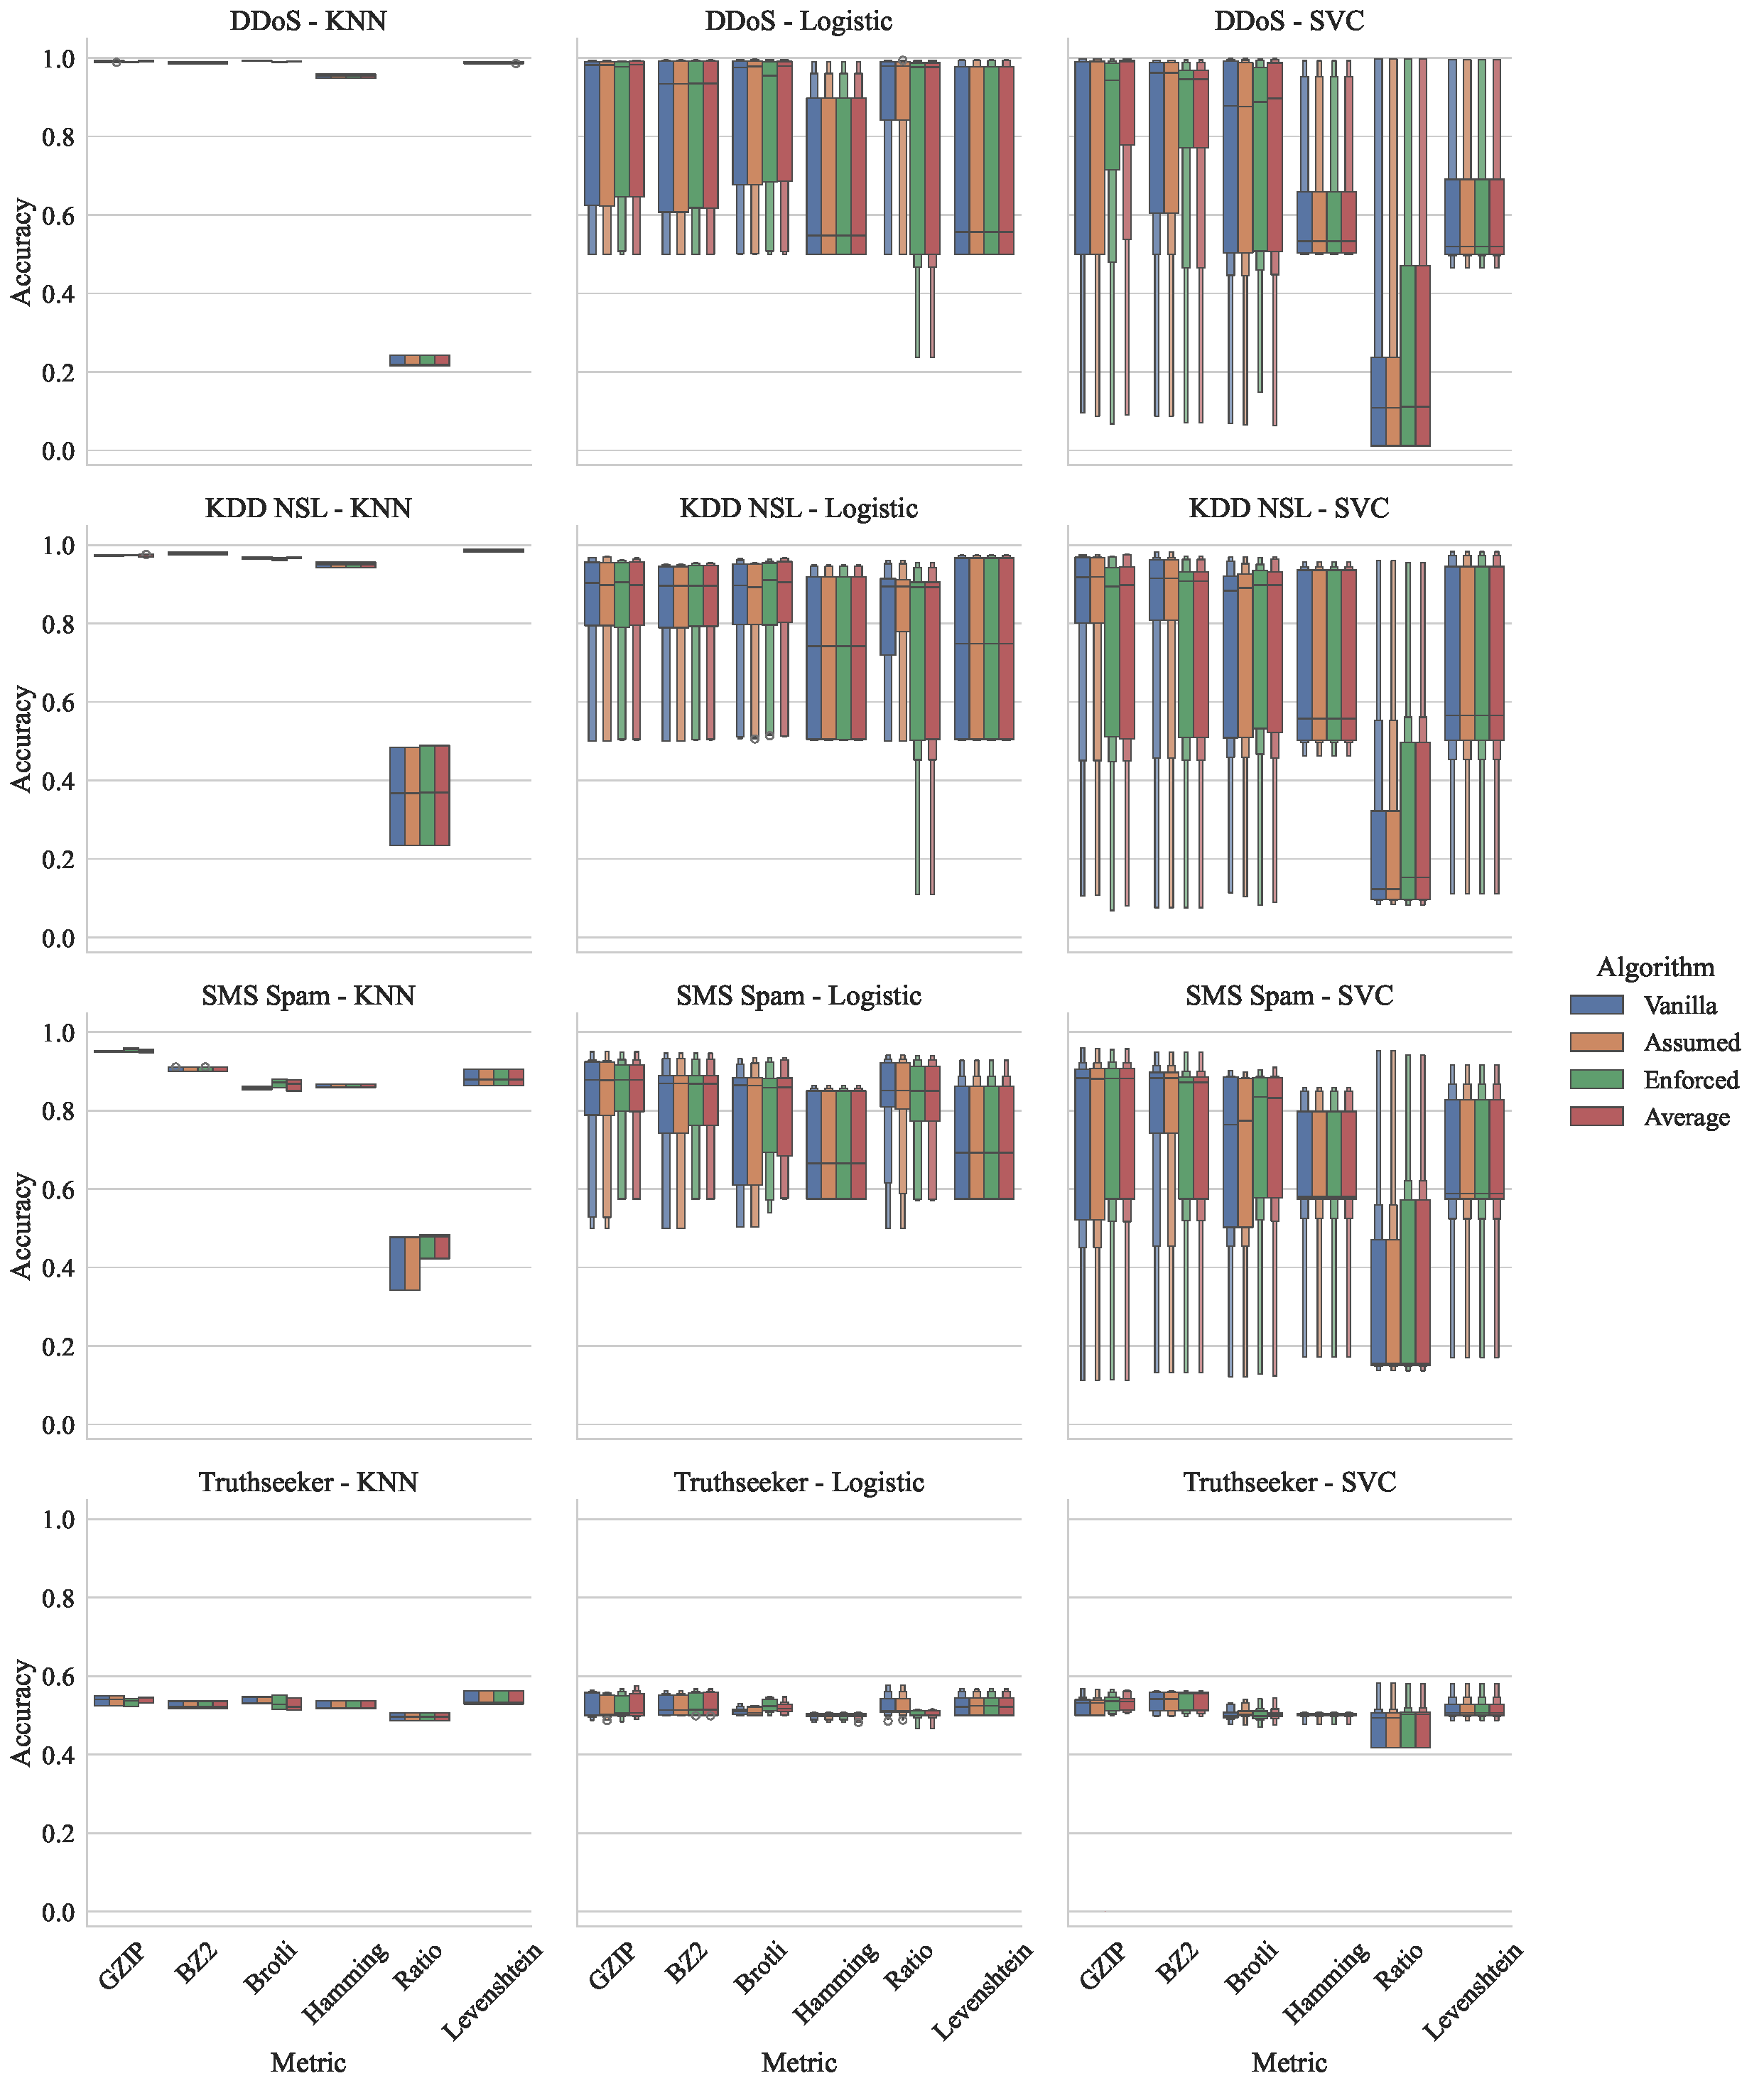
\includegraphics[width=\textwidth]{images/accuracy_vs_algorithm.pdf}
    \caption{The accuracy across each dataset (rows), model (columns) and distance matrix computation algorithm (color) for several different string metrics (x-axis), calculated by averaging the scores of each fold in five-fold cross validation for each set of tested parameters (enumerated in Section~\ref{models}).}
    \label{fig:metric_acc}
\end{figure*}

Figure~\ref{fig:metric_acc} shows the performance of the various classifiers (KNN, logistic, SVC) across each of the datasets using various string metrics to calculate NCD.
NCD using various compressors outperforms the string metrics across all datasets and classifiers.
It is clear that run-times are largely comparable between NCD and various string metrics for both training (Figure~\ref{fig:distance_time}) and inference (Figure~\ref{fig:pred_time}).
Please note that the training step is only necessary for certain configurations of the KNN algorithm and that the vanilla version proposed by Jiang et. al.~\cite{jiang2022less} can skip this step entirely.
Overall, NCD (GZIP, BZ2, Brotli) offers superior performance over the tested string metrics (Hamming, Ratio, Levenshtein) since NCD is more consistently accurate. Across all datasets, the median and peak accuracy of the compressor-based metrics exceeds all the string metrics.



\subsection{Effect of Kernelisation}

\begin{figure*}
    \centering
    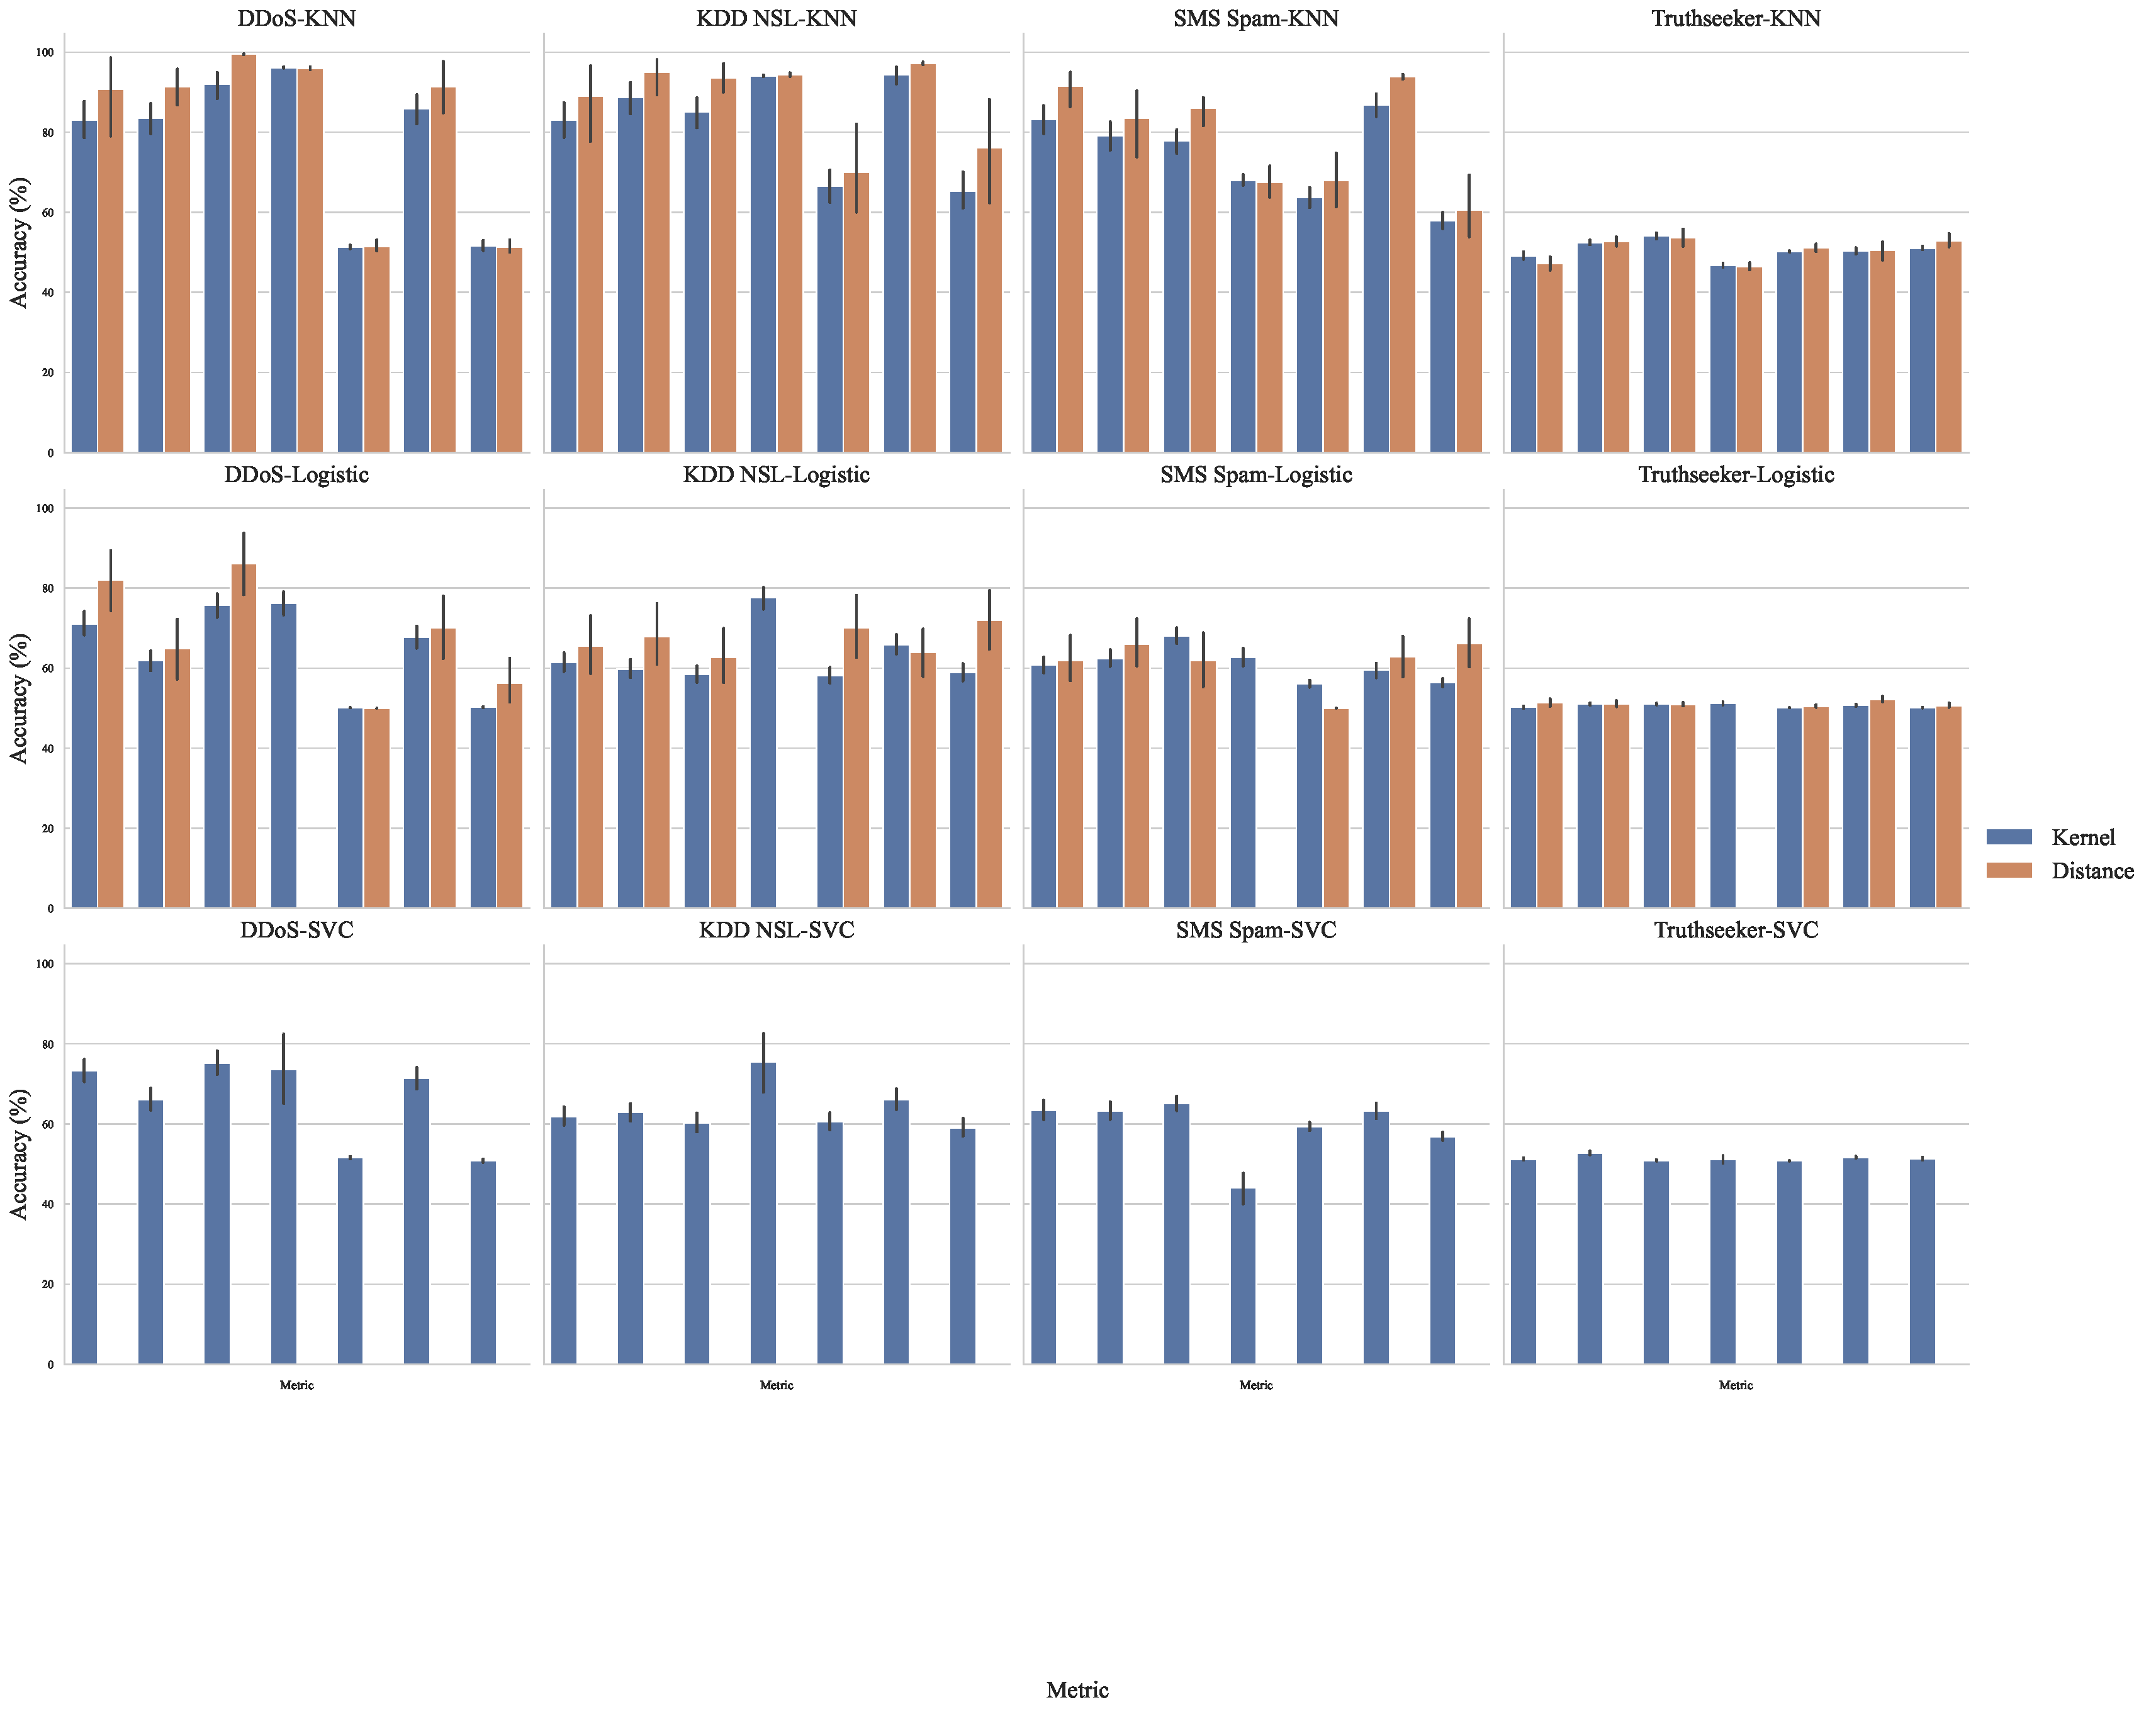
\includegraphics[width=\textwidth]{images/accuracy_vs_kernel.pdf}
    \caption{The accuracy across each dataset (rows), model (columns) and distance matrix computation algorithm (color) for several different kernelisation functions (x-axis), calculated by averaging the scores of each fold in five-fold cross validation for each set of tested parameters (enumerated in Section~\ref{models}).}
    \label{fig:kernel_acc}
\end{figure*}

Figure~\ref{fig:kernel_acc} shows the effect of kernelisation when compared to the un-kernelised distance matrix (on the far right side, denoted with a $D$) across all tested configurations of models across all the datasets.

For KNN, the performance is identical for all datasets and models, which is not unexpected as the chosen kernel functions preserve the order of the neighbours, except when an (erroneous) negative distance occurs.
As the occurrence of negative distances is rare (see Figures~\ref{fig:synthetic_check}~and~\ref{fig:real_world_check}), it is not unexpected that the resulting accuracy remains the same.
KNN performance is consistent across all of the datasets and distance matrix algorithms.

The kernelised logistic regressor fails to outperform the raw distance matrix, on average.
However, after tuning, kernelised logistic regression can also approach perfect accuracy, but the logistic method includes more tuneable parameters, resulting in a longer training time---consistently across all of the datasets and distance matrix algorithms.

Unsurprisingly, the kernelised version of the distance matrix tends to outperform the un-kernelised distance matrix when used to build an SVC since that model is intended to work on similarity metrics (kernels) rather than dissimilarity metrics (distances).
Like with logistic regression, this increased training time comes at the cost of one or more tuneable parameters and the resultant increase in training time.
Nevertheless, SVC might be more appropriate for situations in which the decision boundary is highly complex.
Like with KNN and logistic regression, the performance of SVCs is consistent across all datasets and distance matrix algorithms.


\subsection{Effect of Modified NCD Algorithm}

\begin{figure*}
    \centering
    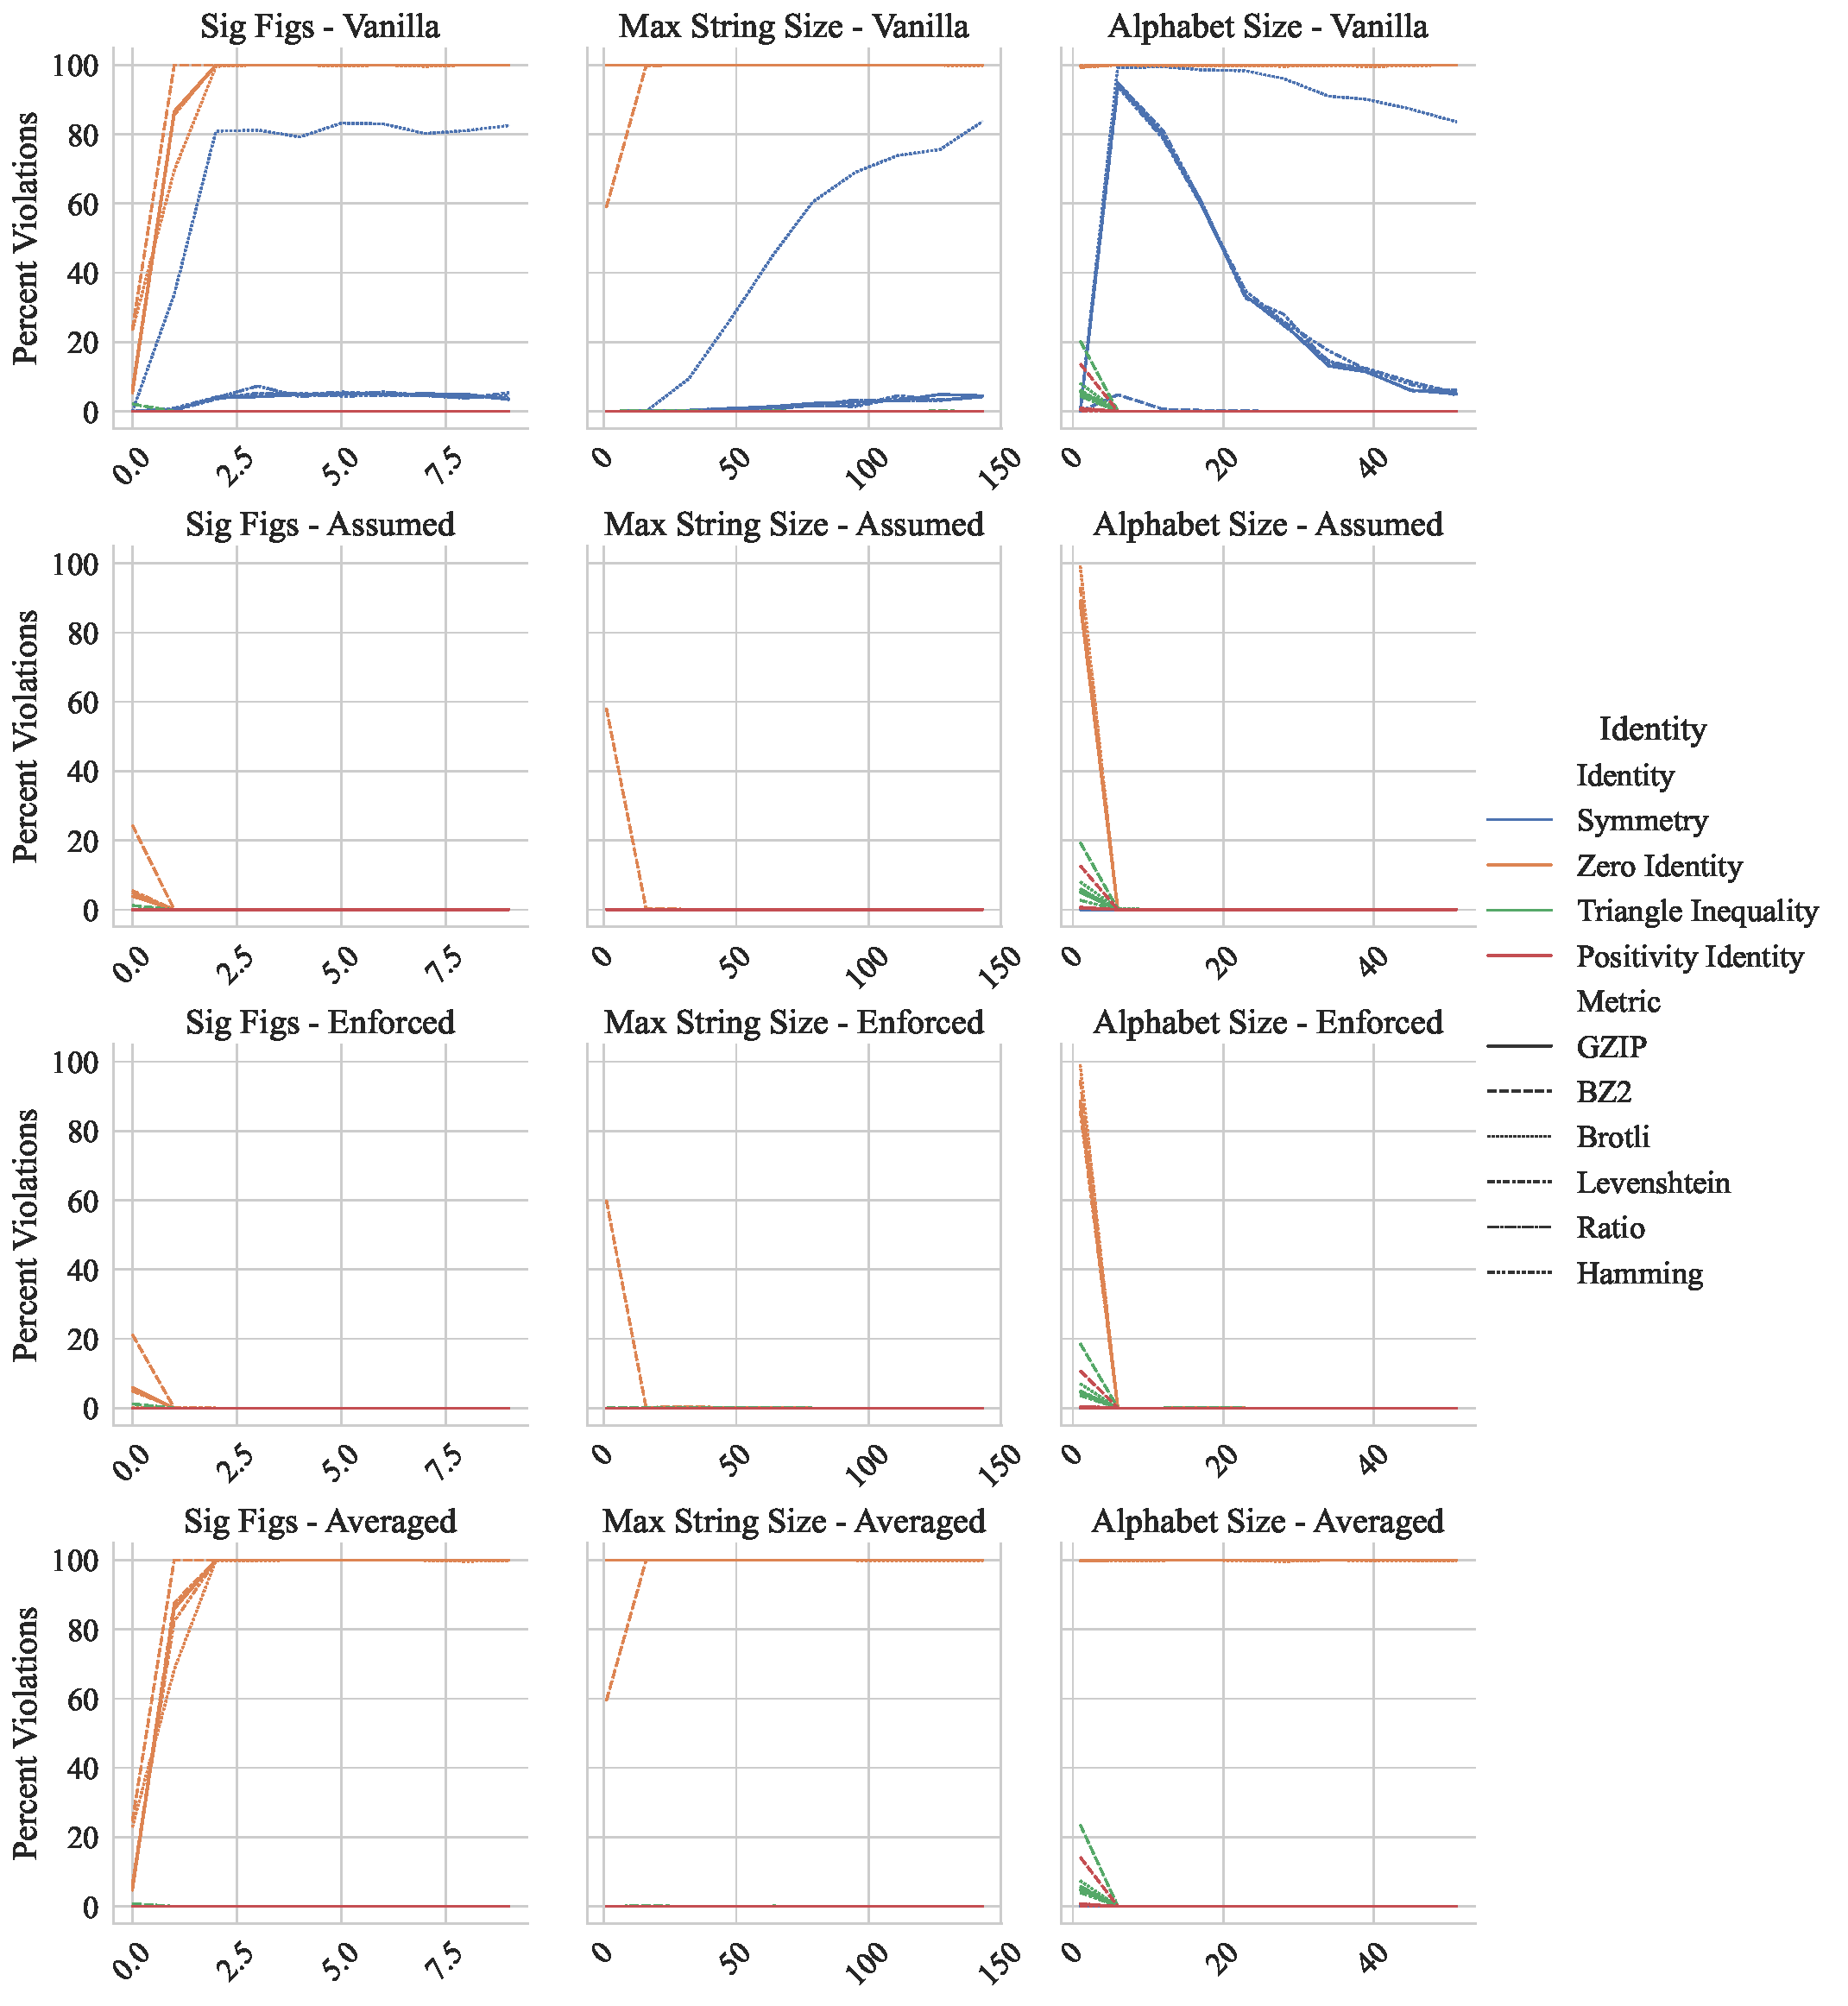
\includegraphics[width=\textwidth]{images/synthetic_check.pdf}
    \caption{
    Percentage of examples found that violate the assumptions outlined in Section~\ref{metric_spaces} using the vanilla (Algorithm~\ref{alg:vanilla}, top row), assumed symmetry (Algorithm~\ref{alg:symmetric}, second row), enforced (Algorithm~\ref{alg:modified}), and averaged (Equation~\ref{eq:average}) algorithms on 100 thousand random strings generated from the standard English alphabet (upper and lowercase).
    \textit{Sig Figs} refers to the number of significant figures. \textit{Max String Size} and \textit{Max Alphabet Size} refer to the number of characters and the number of unique characters respectively.
    Unless otherwise specified by the x-axis in an individual plot, \textit{Max String Size}, \textit{Max Alphabet Size}, and \textit{Sig Figs} were all 144 characters (the character limit of a ``tweet''), 52 letters (upper and lower case English letters), and 10 significant figures. Each colour corresponds to a different axiom as defined in Section~\ref{metric_spaces} and each line marker corresponds to a different string distance as outlined in Section~\ref{compressors} and Section~\ref{string_metrics}. \cm{Here it says positivity instead of non-negativity, but that has been fixed locally and will be re-rendered when the ongoing experiments finish.}
    }
    \label{fig:synthetic_check}
\end{figure*}

\begin{figure*}
    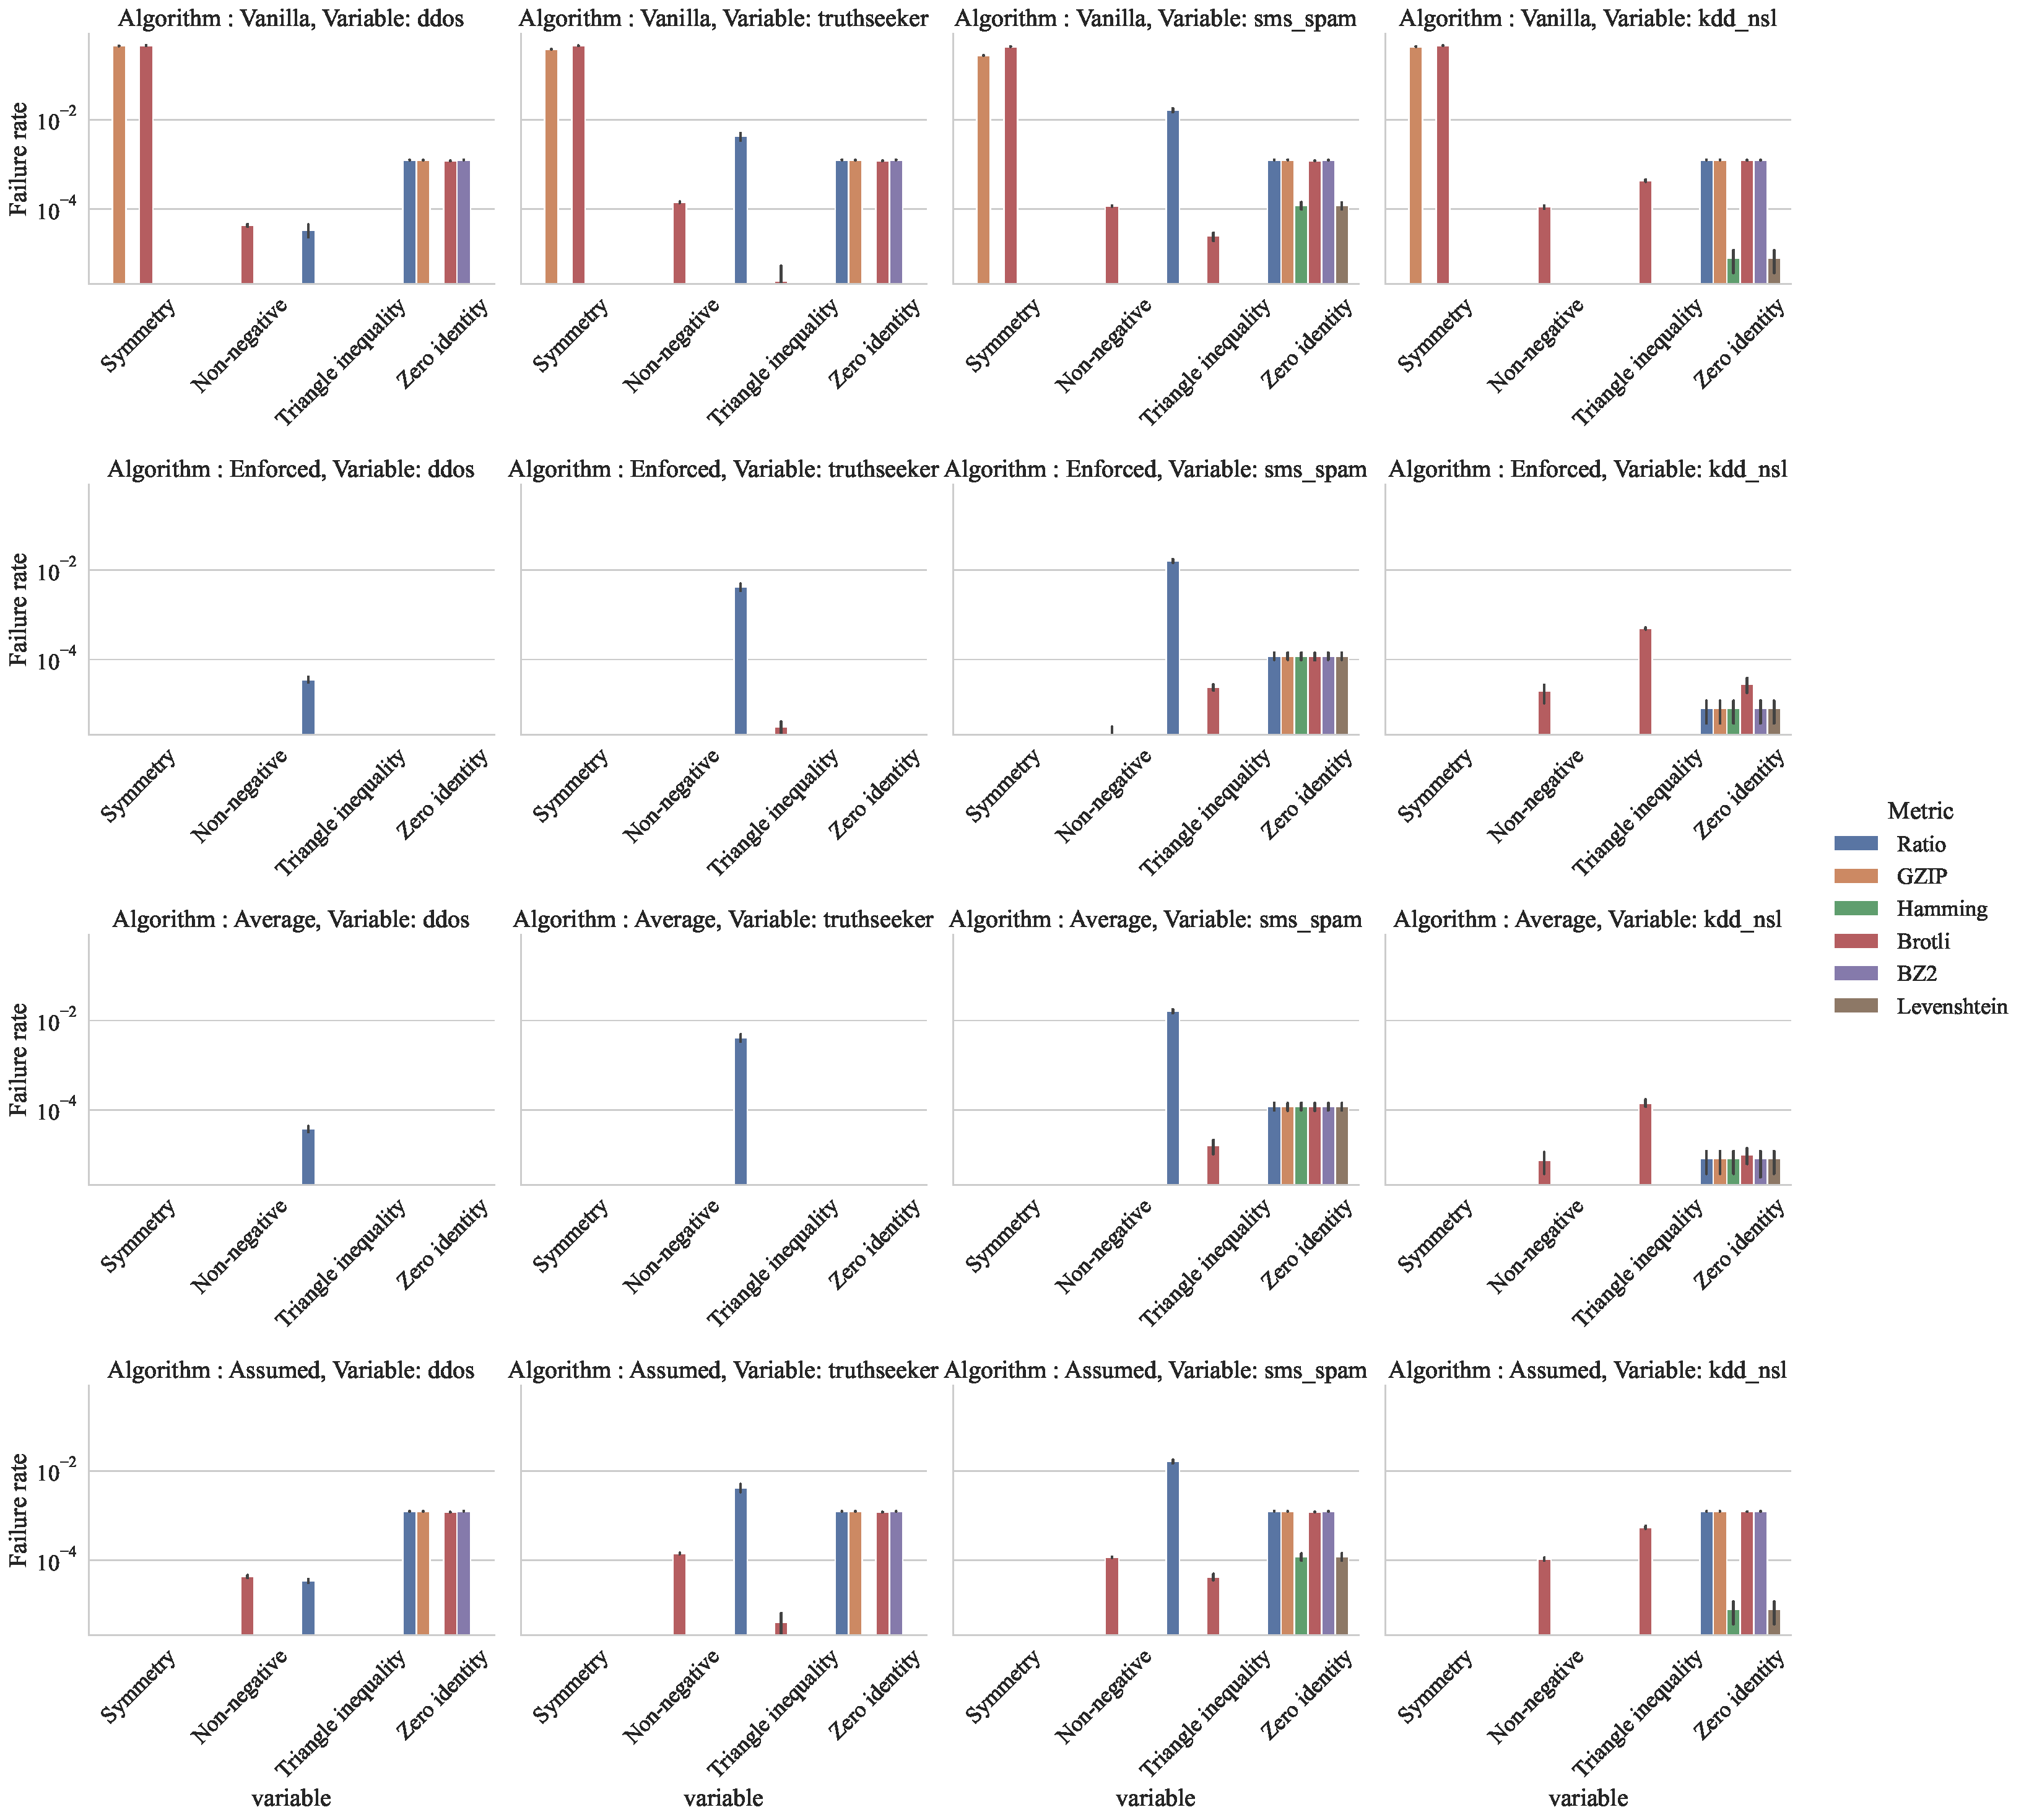
\includegraphics[width=\textwidth]{images/read_world_check.pdf}
    \caption{Percentage of examples found that violate the assumptions outlined in Section~\ref{metric_spaces} using the vanilla (Algorithm~\ref{alg:vanilla}, top row), assumed symmetry (Algorithm~\ref{alg:symmetric}, second row), enforced (Algorithm~\ref{alg:modified}), and averaged (Equation~\ref{eq:average}) algorithms on the training matrices for each of the outlined datasets. Each column is dedicated to a dataset and each model is given a column. The x-axis displays which of the axioms is violated and the colour indicates which distance matrix algorithm was used. Since evaluating all possible distance 3-tuples would be computationally infeasible for even hundreds of samples, three disjoint distances were sampled  100 thousand times. \cm{Note: I have fixed the capitalisation in this plot, but am waiting on the new results after changing the ratio metric before re-rendering.}}
    \label{fig:real_world_check}
\end{figure*}

Figures~\ref{fig:metric_acc}~and~\ref{fig:kernel_acc} depict the accuracy (top), Figure~\ref{fig:distance_time} depicts the   training time per sample, and Figure~\ref{fig:pred_time}  depicts the inference time per sample (bottom) for each algorithm (denoted by colour and outlined in ~\ref{extensions}).
The accuracy of the modified algorithm is fairly consistent with the unmodified version.
In practice, the model builder would choose the most accurate model, which is consistent across the algorithms and classifiers for each dataset.
However, the modified version of the algorithm is clearly much faster per sample when constructing the distance matrix ($t_t$) by reducing the number of distance computations by a factor of around 2.
This comes at the marginal cost of a few hundred milliseconds for each prediction, however, but this could easily be mitigated by skipping the algorithmic modifications during the prediction step and handle the problem of negative distances at run-time, depending on the particular application.
Overall, it is clear that this modified version of NCD offers significant run-time improvements while costing nothing in terms of accuracy.
Additionally, by running the vanilla version during prediction and using the modified version if and only if the training distance matrix is calculated, these downsides can be avoided entirely.
% However, that may produce distance matrices that are incompatible with other tooling or models (see: Figure~\ref{fig:synthetic_check}, middle row), most of these are mitigated with the proposed modifications (see: Figure~\ref{fig:synthetic_check}, bottom row).
% However, two classes of counterexamples remain.
% The first occurs with very short strings
% $NCD("ABB", BBBB) =0$ because the marginal length associated with the repeated ``BB'' token happens to be the exact length as the marginal length associated with the token ``A''.
% This second occurs for the triangle inequality.
% Letting $x =AACAABC$, $ y = AA$, and $
% z=AAA$, we find that $NCD(x,y) \approx .26$ while $NCD(x,z) + NCD(z,y) \approx .23$, but it's not clear that this is a problem in the theory. Including the string ``AAA'' provides additional context that ``AA'' may have a distinct meaning apart from ``A'' repeated twice which is why the distance of the sum \textit{is} less than the distance between $x$ and $z$. Additionally, it doesn't seem to be a problem in practice.
% As the max string size or the maximum alphabet size is increased, these problems quickly disappear(see: Figures~\ref{fig:synthetic_check}~and~\ref{fig:real_world_check}.



\subsection{Run-time Considerations}

Figure~\ref{fig:distance_time} depicts the time needed to calculate the distance matrix per sample in the training set for each dataset (column), algorithm (colour) and metric (x-axis).
It is clear that the run-times of the metrics are fairly consistent across the datasets and that the proposed run-time improvements (denoted ``Assumed'' and ``Enforced'') do decrease the distance matrix calculation time with no resulting loss in accuracy (see: Figure~\ref{fig:metric_acc}).
While the symmetric extension of NCD (denoted ``Averages'') does take significantly more time than the other distance matrix algorithms, that marginal increase is mere milliseconds in practice and is guaranteed to be symmetric without assuming or enforcing symmetry.
However, Hamming distance takes significantly more time than other metrics on the DDoS dataset and GZIP takes significantly more time than other metrics on the KDD NSL dataset.
This effect can be mitigated by considering the run-time costs during the model training stage since these metrics take longer but do not result in significantly better accuracies (see: Figure~\ref{fig:metric_acc}) for those datasets.

Figure~\ref{fig:train_time} depicts the time needed to train a given model on a given distance matrix and the time need to calculate the distance matrix on 800 training samples (64 thousand pairwise distances) is depicted in Figure~\ref{fig:train_time}.
The training step can be skipped entirely if the decision boundary can be accurately modelled by an unweighted KNN algorithm, but the distance matrix calculation must still occur for prediction.
Overall, training times (the combination of Figure~\ref{fig:distance_time}~and~\ref{fig:train_time}) are low enough that this could feasibly be deployed on a user's device without specialised hardware (which is generally not true for neural networks).
If we pessimistically assume a training time of 50 milliseconds per sample, then training could occur as the user (or router or antivirus software or social media algorithm) encounters the sample in real-time with a latency that would be unnoticeable to most humans (on the order of a  few hundred milliseconds, depending on age and other factors~\cite{reaction_time}).

Figure~\ref{fig:pred_time} depicts the time needed to predict a new classification on a single sample for each dataset (row), classifier (column), algorithm (colour) and metric (x-axis).
The prediction time per sample (after calculating the distance between a new sample and those in the training set) is trivial across all distance matrix algorithms, datasets, models, and metrics, though the branching logic introduced by the ``Assumed'' and ``Enforced'' algorithms does increase the model latency by a fraction of a millisecond.
Overall, it is clear that the run-time improvements are effective and that NCD is can be plausibly used in real-time, client-side settings.
It is clear that the time needed to do the compression is a larger factor in the resulting run-time than either the model training or model prediction, though models with many hyper-parameters would need to be tuned for each user and this run-time can be significant.
Rather than tuning a model every time an application is launched or a webpage is refreshed, the resulting model parameters could be stored locally.
This increases the attack surface, but only for that particular user.
Since passwords, banking information, authentication tokens, and other secrets are stored in this manner, this is unlikely to be objectionable to users---especially since the attack surface is significantly reduce compared to something like a neural network.
In applications where latency is more important than privacy, then the distance matrix can be pre-computed (\textit{e.g.} on a email server) reducing the run-time and computational costs for the user.
In applications where privacy is more important than latency, this task can run in the background, as users receive new messages or content and before they launch the application.
% Since content on the internet is often sent in a compressed form~\cite{} and decompressed for the user, calculating the un-concatenated length of the compressed content (\textit{e.g.} $C(x), C(x')$) is trivial in practice, reducing model overhead.


% cosine similarity + classifiers: https://www.tandfonline.com/doi/full/10.1080/08839514.2020.1723868#d1e195 This paper uses a cosine distance to yield a run-time of O(m+n) since encoding the string as an n-gram is much more expensive than the cosine calculation, but only needs to be done once per sample rather than once per pairwise distance.


\begin{figure*}
    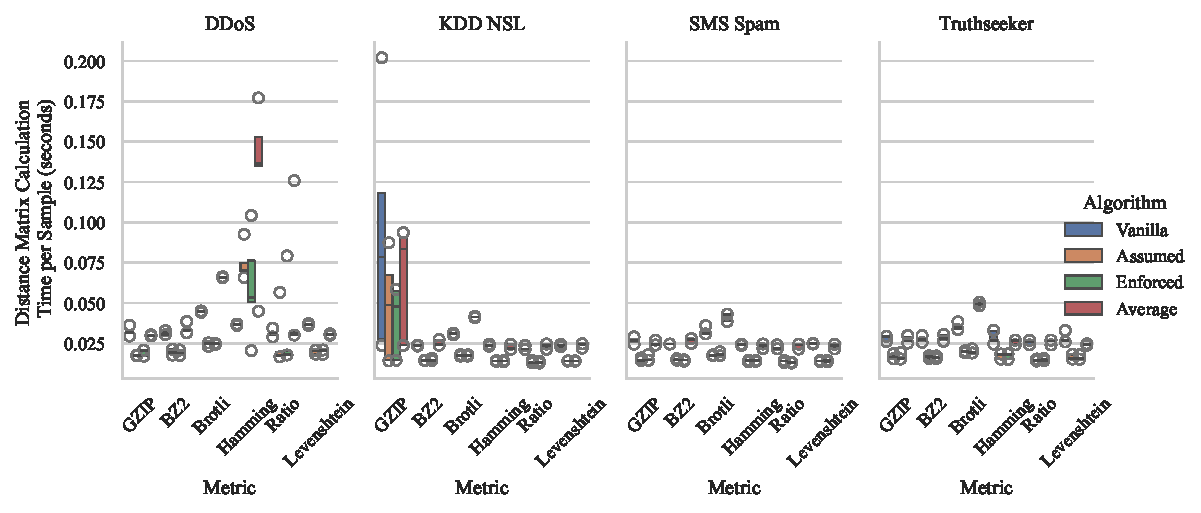
\includegraphics[width=\textwidth]{images/distance_matrix_time_vs_algorithm.pdf}
    \caption{The distance matrix calculation time per sample for each metric (x-axis), dataset (columns) and algorithm (colour). Because the distance matrix was only calculated once per dataset/algorithm/metric combination there is no differentiation between the models.}
    \label{fig:distance_time}
\end{figure*}

\begin{figure*}
    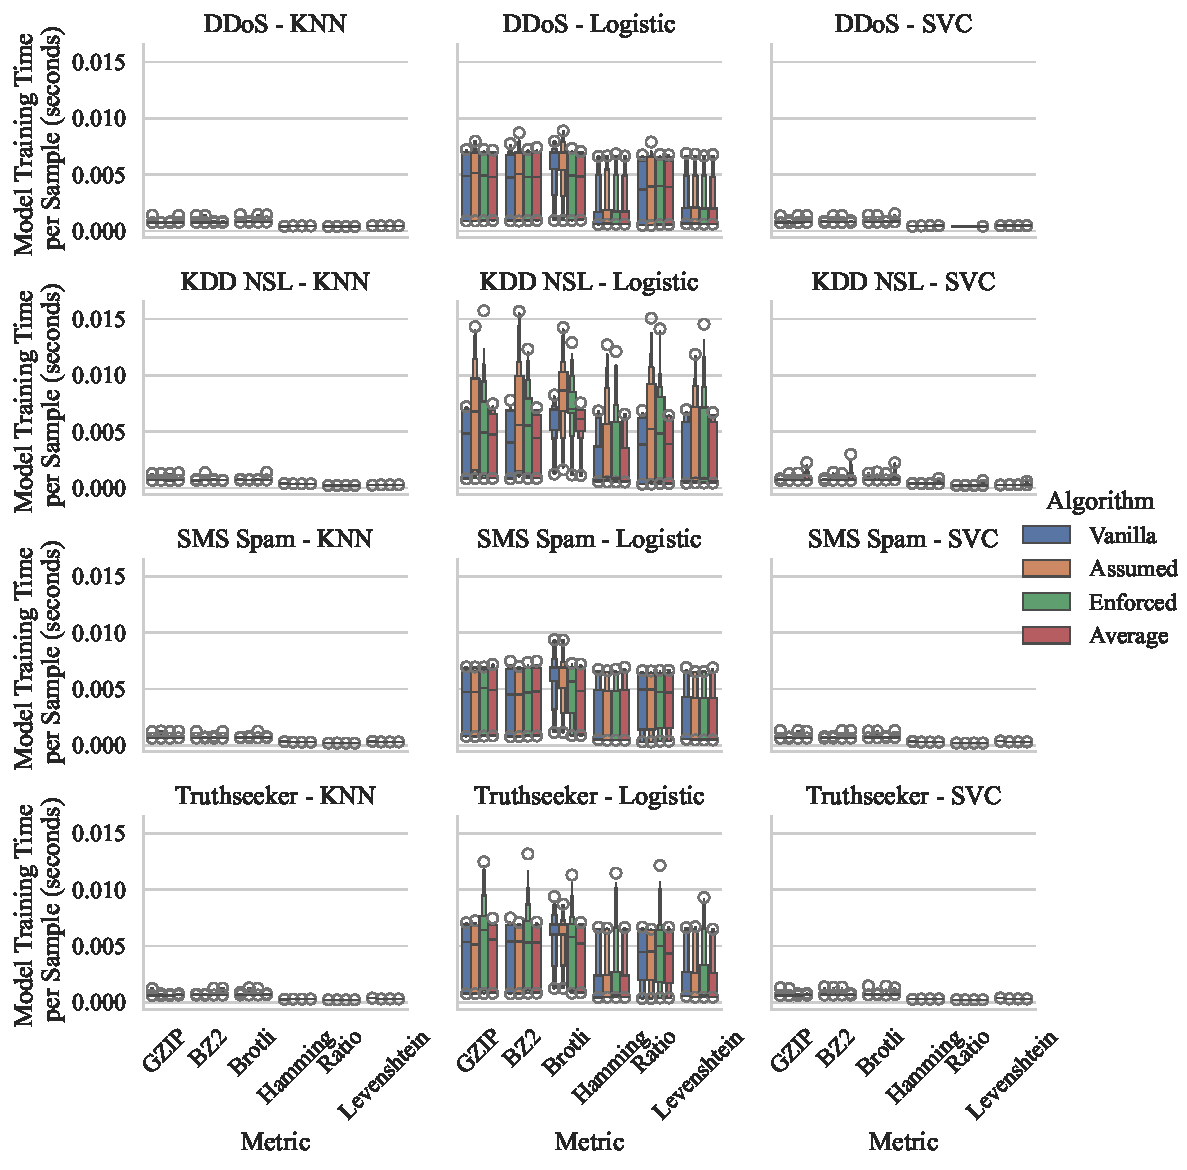
\includegraphics[width=\textwidth]{images/train_time_vs_algorithm.pdf}
    \caption{The training time  per sample (after computing the distance matrix) for each metric (x-axis), dataset (rows), model (columns) and algorithm (colour).}
    \label{fig:train_time}
\end{figure*}

\begin{figure*}
    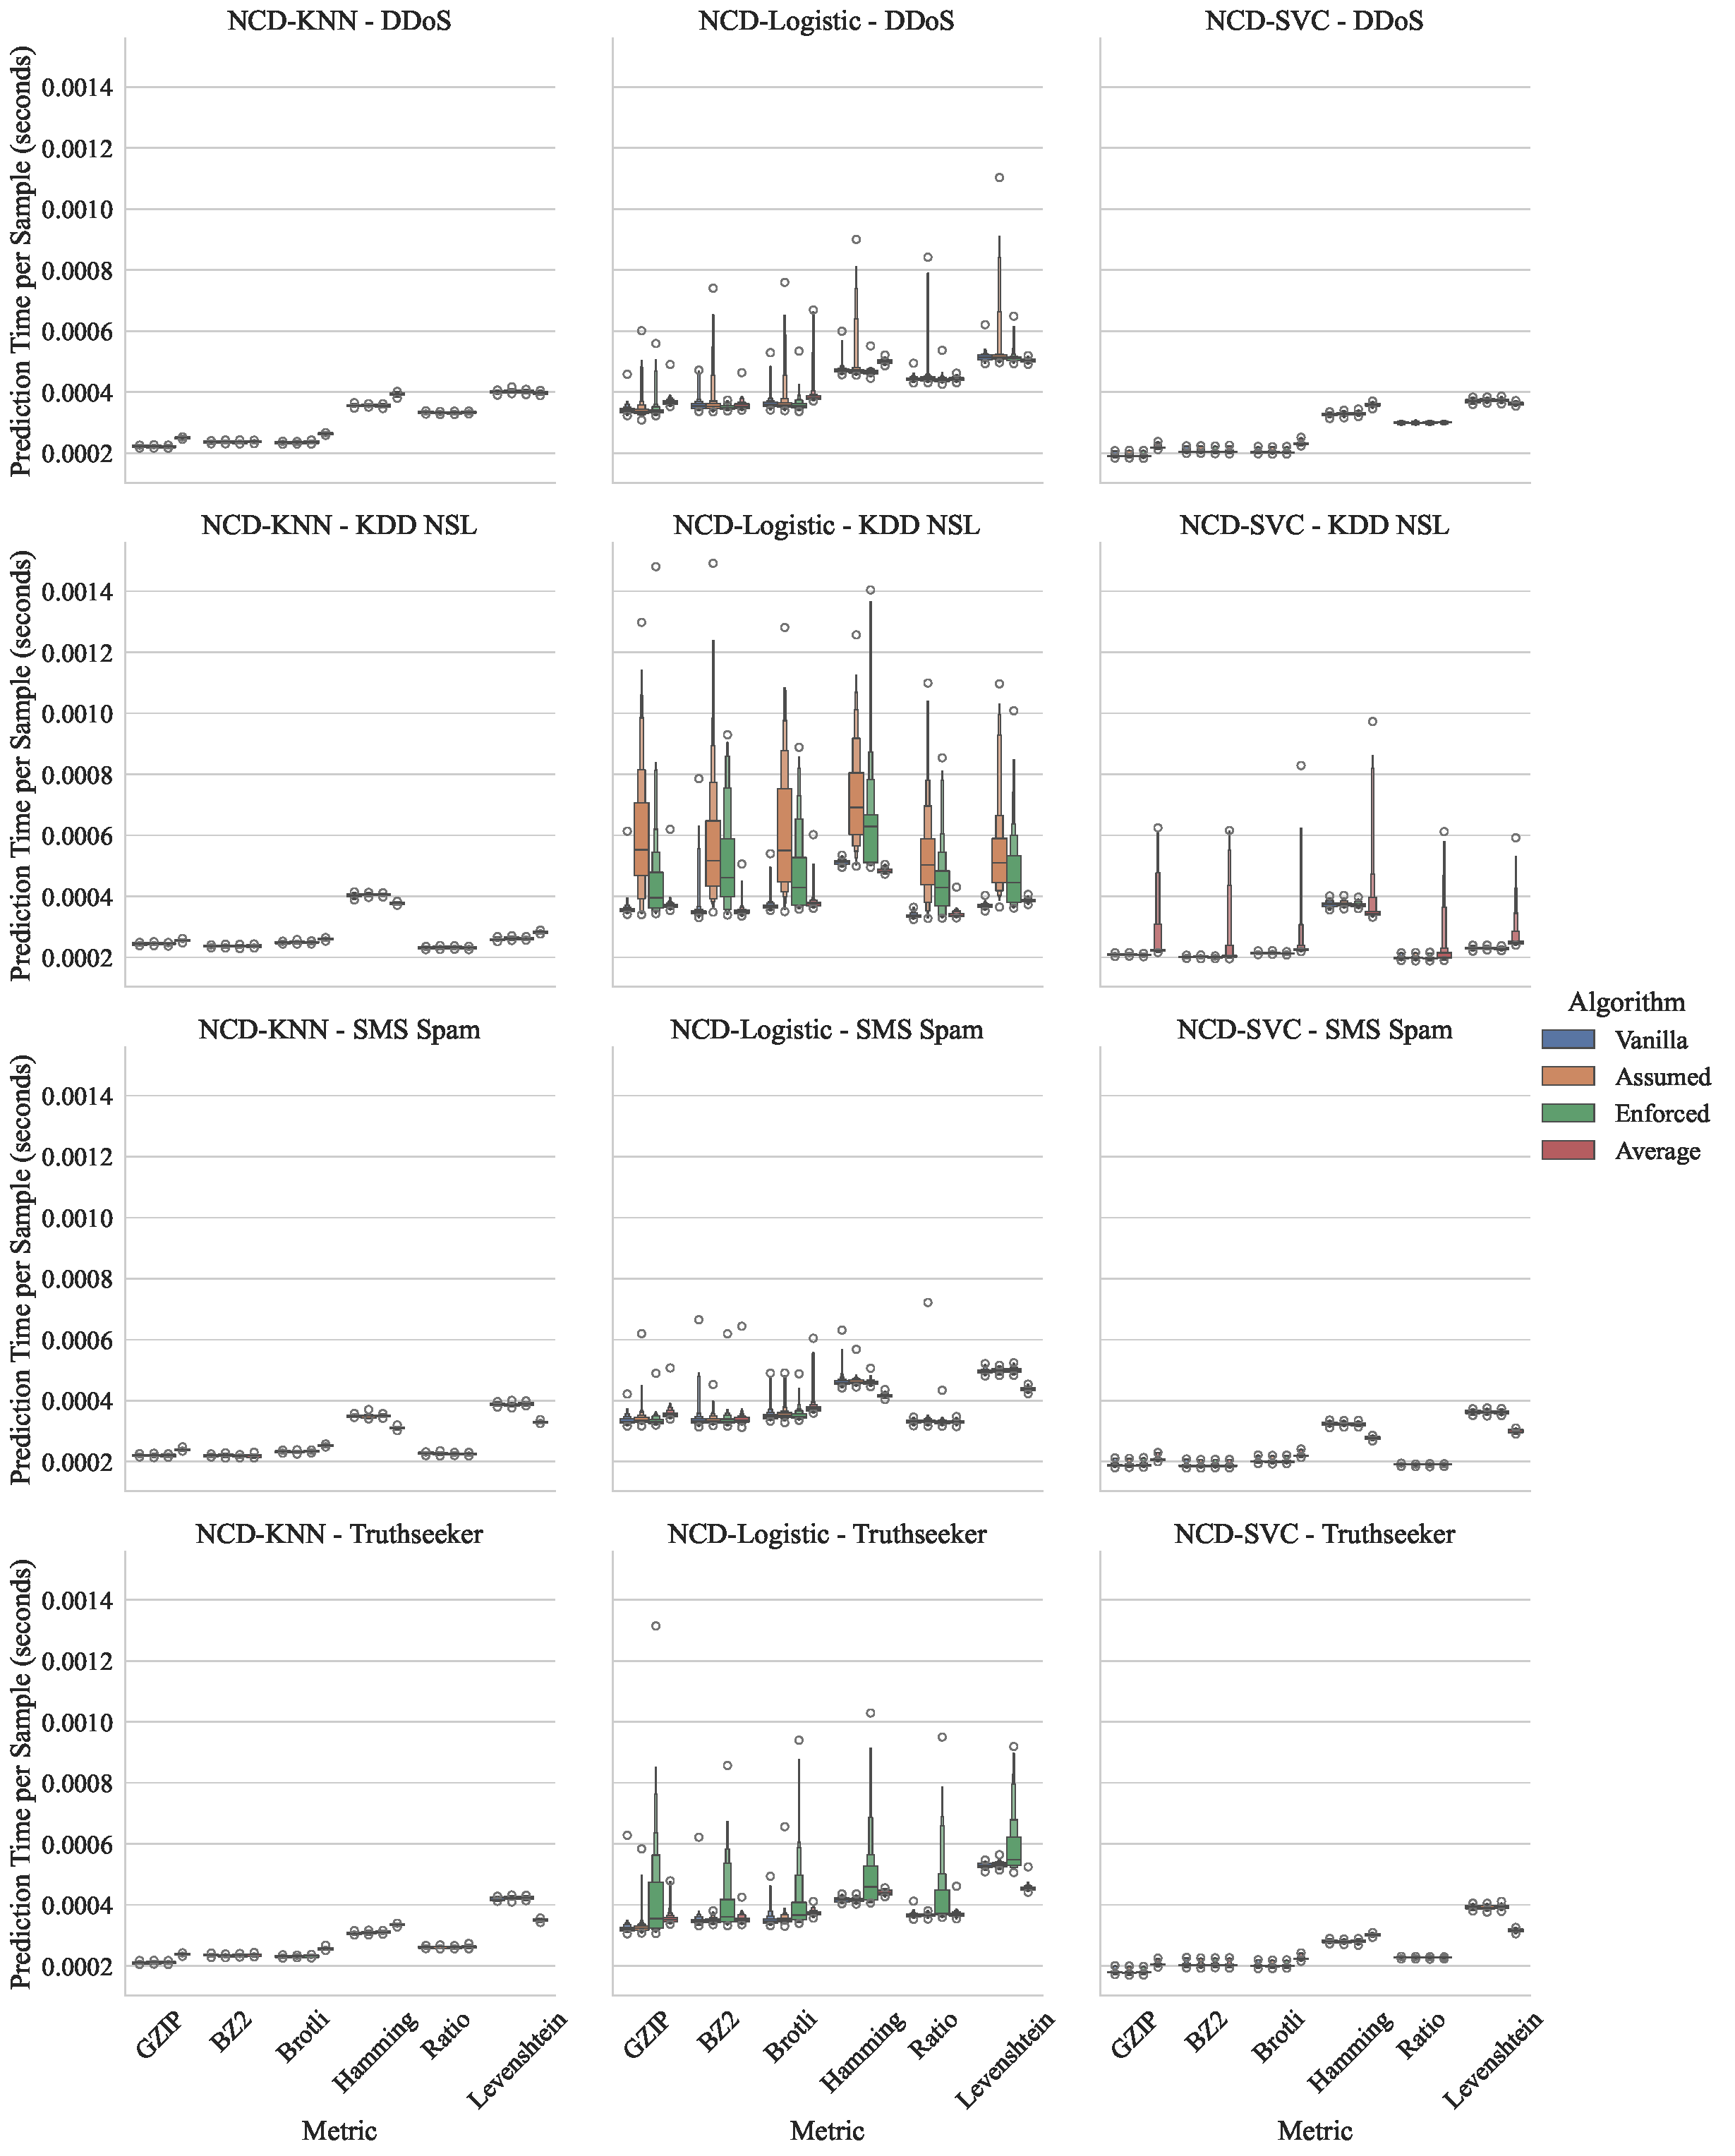
\includegraphics[width=\textwidth]{images/pred_time_vs_algorithm.pdf}
    \caption{The predictions time per sample (after computing the distance matrix) for each metric (x-axis), dataset (rows), model (columns) and algorithm (colour).}
    \label{fig:pred_time}
\end{figure*}

\subsection{Sample Size Considerations}
Figure~\ref{fig:sample_size} depicts the accuracy of the best-performing model (\textit{e.g.} the model tuned via cross-validation) for each dataset (rows), model (columns), metric (line style), and algorithm (colour) for a number of different sample sizes (x-axis) using 200 samples that were not used during cross-validation.
It is clear that this method is quite effective even on 10s of samples and that the accuracy tends to converge quickly across datasets, models, metrics, and distance matrix algorithms.
\begin{figure*}
    \centering
    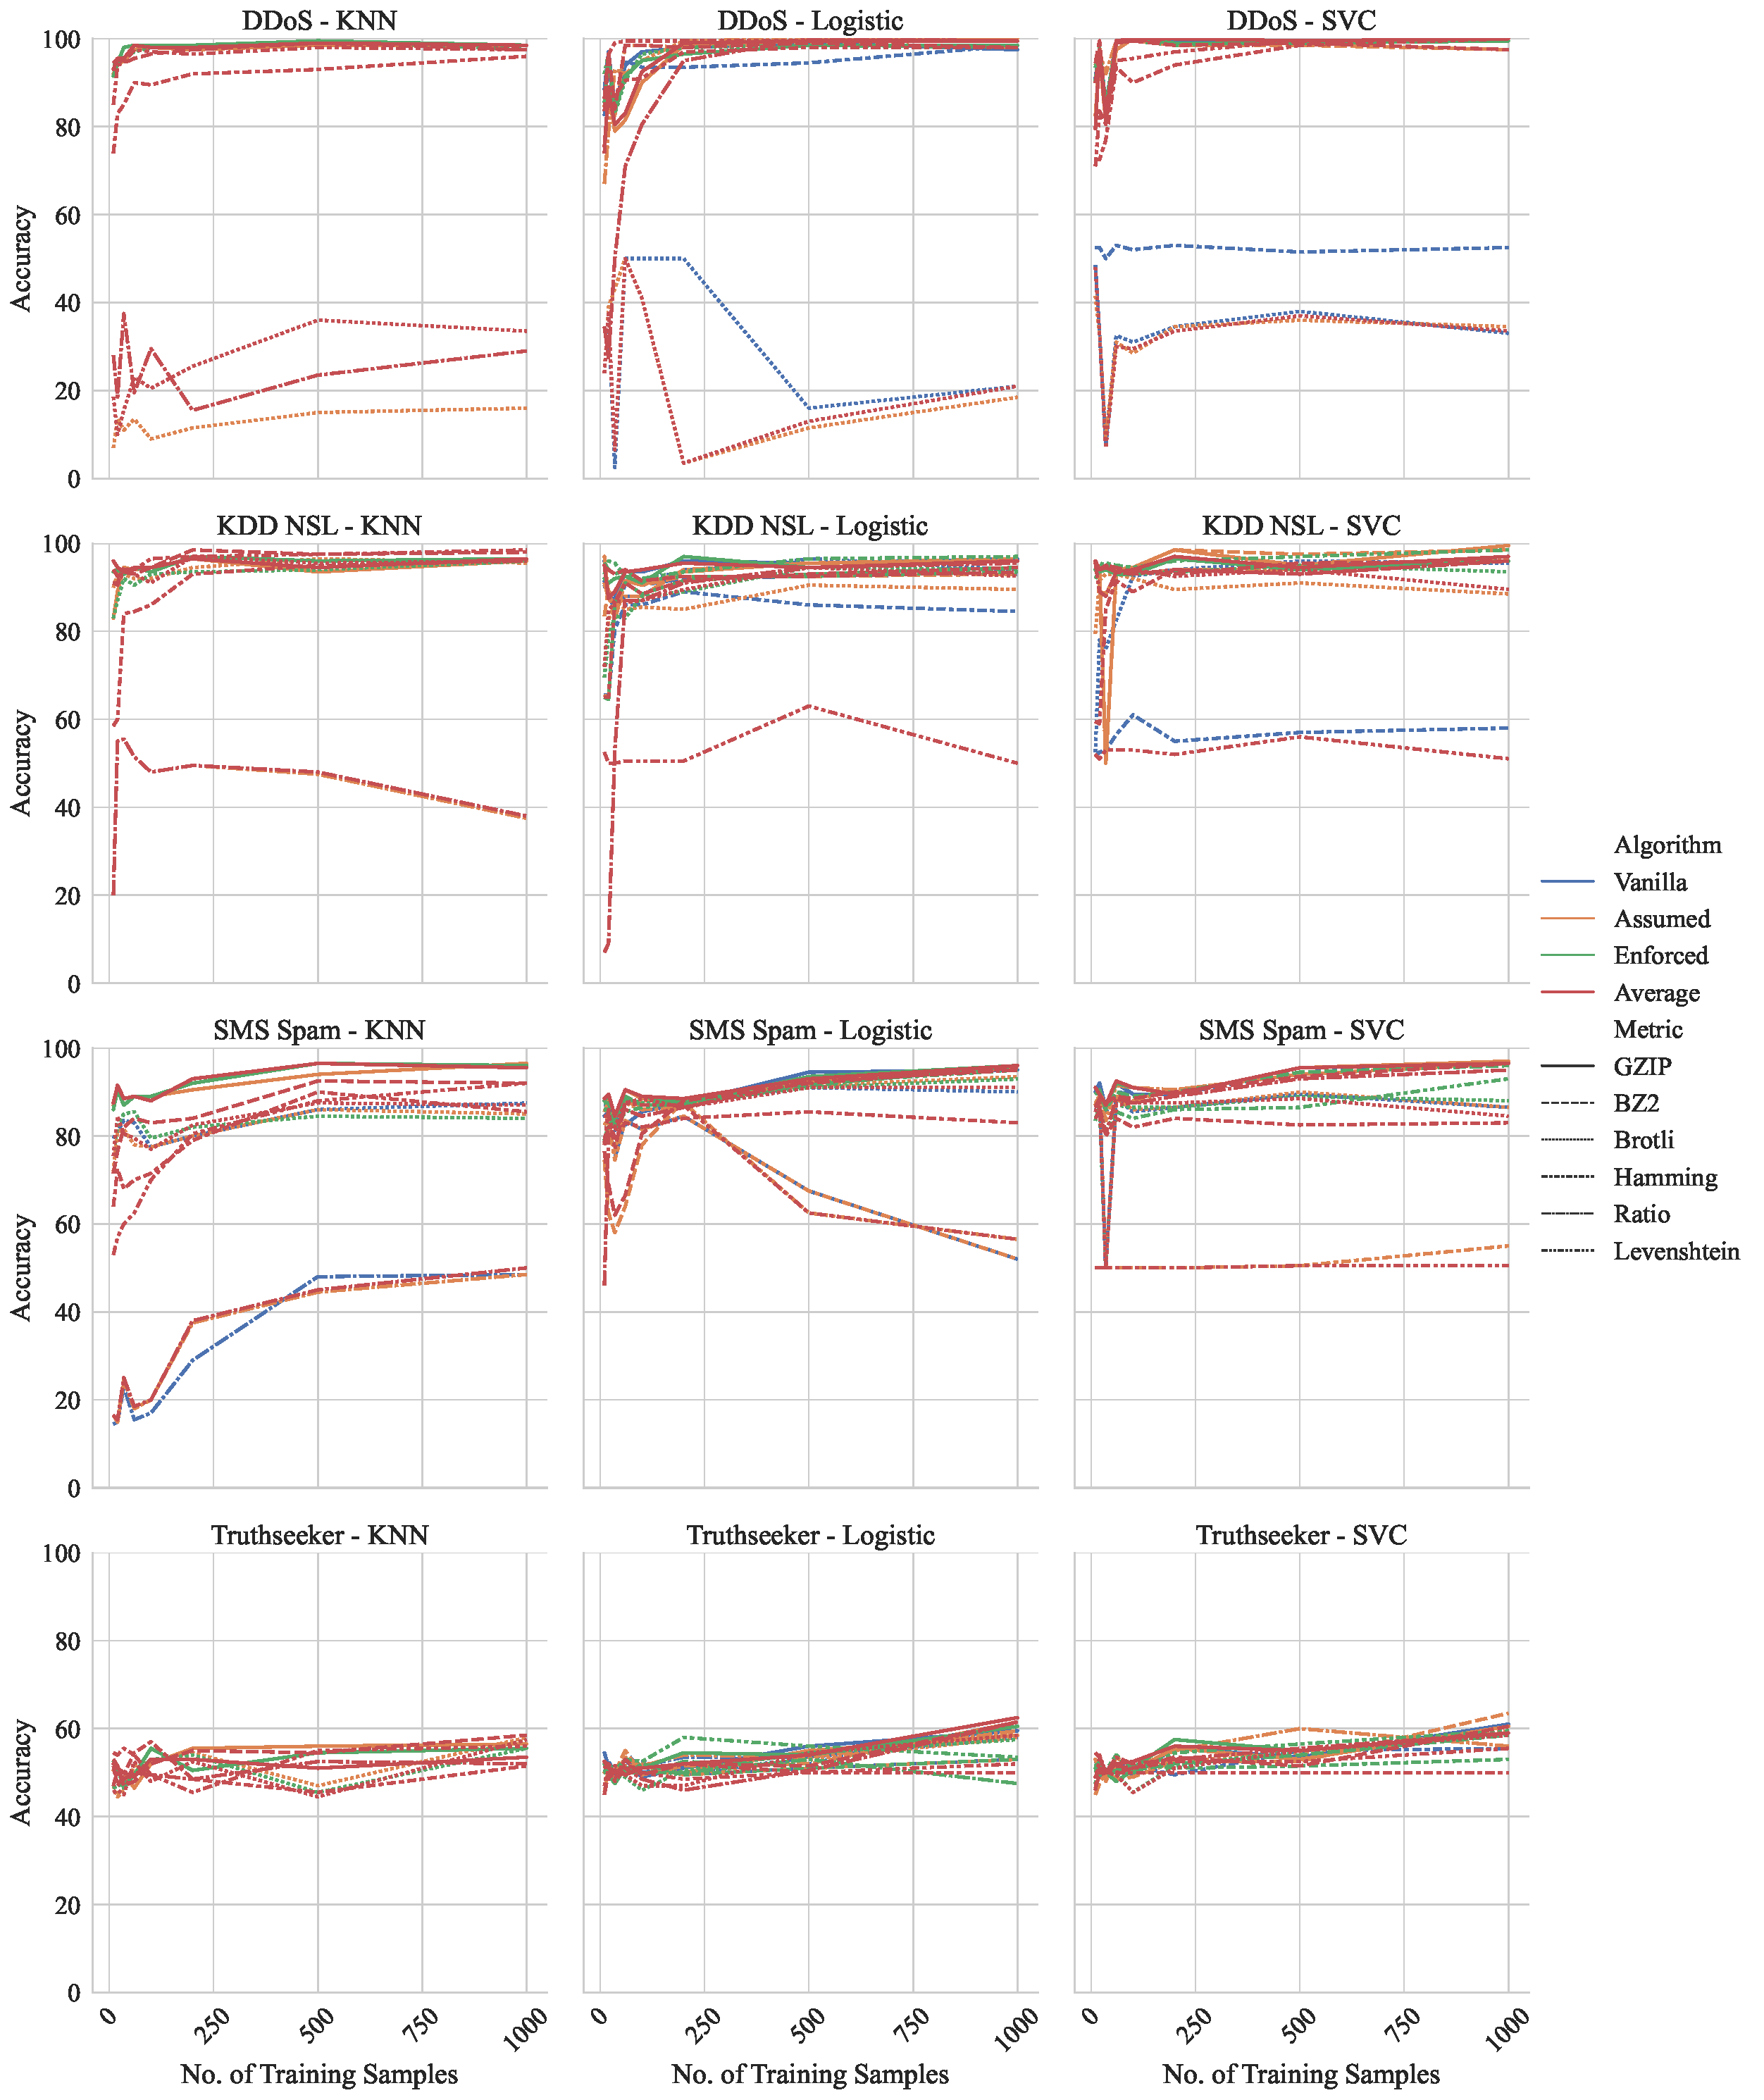
\includegraphics[width=\textwidth]{images/accuracy_vs_train_size.pdf}
    \caption{The accuracy for each metric (line style), dataset (rows), model (column) and algorithm (colour) as the number of training samples varies (x-axis) computed on 200 samples that were withheld from the cross-validation step (as reported in Figures~\ref{fig:kernel_acc}~and~\ref{fig:metric_acc})}
    \label{fig:sample_size}
\end{figure*}

\section{Considerations}
\label{considerations}
While the proposed algorithm (see \ref{alg:modified}) does improve upon certain edge cases outlined in Section~\ref{pseudometric}, the examined condensing methods (see: Section~\ref{extensions} do not have any significant effect on model performance (see: Figures~\ref{fig:metric_acc}~and~\ref{fig:kernel_acc}).
However, the vanilla NCD-KNN proposed by Jiang et. al.~\cite{jiang2022less} remains an effective choice if the training step is deemed too expensive for the chosen applications and the only reason to deploy the extensions would be to reduce the training time--- an unnecessary step for unweighted KNN.
Here, the authors would like to note the borderline performance of all metrics on the Truthseeker dataset---both NCD and more traditional distance measures.
However, this is on par with the performance from the original authors~\cite{truthseeker}.
To the best knowledge of the authors, most content on the platform formerly known as Twitter is simply indistinguishable from bot-generated spam---using any known distance metric.
\cm{TODO discuss the new threat model  and the limitations of browser-based security (e.g. XSS attacks). Also discuss concerns around censorship/surveillance and how the labels must be generated by users and not platform operators so as to decentralise the power of labelling something as malicious (e.g. if enough users mark you as spam, then Facebook marks you as spam rather than Facebook deciding a priori what spam is.)}
% cosine similarity + classifiers: https://www.tandfonline.com/doi/full/10.1080/08839514.2020.1723868#d1e195 This paper uses a cosine distance to yield a run-time of O(m+n) since encoding the string as an n-gram is much more expensive than the cosine calculation, but only needs to be done once per sample rather than once per pairwise distance.
\section{Conclusion}
\label{conclusion}

It is clear from Figures~\ref{fig:metric_acc}-\ref{fig:distance_time} that the modified distance matrix algorithms proposed in this work are superior to the method proposed by Jiang et. al. when applied used a distance measure for kernelised classifiers.
By pre-emptively handling cases that would result in negative values for distance (thus violating the Non-negativity axiom) and sorting the inputs, this modified NCD is guaranteed to behave more like a true metric.
By inducing a metric that is more proper, the model builder can use standard tooling (e.g.~\texttt{scikit-learn}) to build classifiers that perform well on an exceedingly small number of samples.
The end result is a real-time, client-side classification algorithm that does not rely on federation, centralization, or the large scale processing of millions of data points across a global user-base.
By training a model for each user, session, and/or device, poisoning attacks~\cite{biggio_poisoning_2013} are categorically avoided.
Furthermore, this reduces the attack surface of attacks like model inference attacks, database exfiltration attacks, and evasion attacks since a malicious user would need to target the personalised classifier of each user~\cite{biggio_evasion_2013,deepfool,chakraborty_adversarial_2018}.
While it is known that some attacks are quite transferable~\cite{wang2021enhancing}, this reduces the common attack surface to \textit{only} the samples that are universal across the user base and a new model can be generated trivially by refreshing the page or appending the offending sample to the labelled (training) dataset.

%% The Appendices part is started with the command \appendix;
%% appendix sections are then done as normal sections
% \appendix

% \section{Sample Appendix Section}
% \label{sec:sample:appendix}
% Lorem ipsum dolor sit amet, consectetur adipiscing elit, sed do eiusmod tempor section \ref{sec:sample1} incididunt ut labore et dolore magna aliqua. Ut enim ad minim veniam, quis nostrud exercitation ullamco laboris nisi ut aliquip ex ea commodo consequat. Duis aute irure dolor in reprehenderit in voluptate velit esse cillum dolore eu fugiat nulla pariatur. Excepteur sint occaecat cupidatat non proident, sunt in culpa qui officia deserunt mollit anim id est laborum.

%% If you have bibdatabase file and want bibtex to generate the
%% bibitems, please use
%%
 \bibliographystyle{elsarticle-num}
 \bibliography{bibliography}

%% else use the following coding to input the bibitems directly in the
%% TeX file.

% \begin{thebibliography}{00}

% %% \bibitem{label}
% %% Text of bibliographic item

% \bibitem{}

% \end{thebibliography}
\end{document}
\endinput
%%
%% End of file `elsarticle-template-num.tex'.
